%% 
%% Copyright 2019-2020 Elsevier Ltd
%% 
%% This file is part of the 'CAS Bundle'.
%% --------------------------------------
%% 
%% It may be distributed under the conditions of the LaTeX Project Public
%% License, either version 1.2 of this license or (at your option) any
%% later version.  The latest version of this license is in
%%    http://www.latex-project.org/lppl.txt
%% and version 1.2 or later is part of all distributions of LaTeX
%% version 1999/12/01 or later.
%% 
%% The list of all files belonging to the 'CAS Bundle' is
%% given in the file `manifest.txt'.
%% 
%% Template article for cas-sc documentclass for 
%% double column output.

%\documentclass[a4paper,fleqn,longmktitle]{cas-sc}
\documentclass[a4paper,fleqn]{cas-sc}

% \usepackage[numbers]{natbib}
%\usepackage[authoryear]{natbib}
\usepackage[square,numbers]{natbib}
\usepackage{graphicx}
\usepackage{subcaption}
\usepackage{caption}
\usepackage{bm}
\usepackage{algorithmic}
\usepackage{hyperref}
\usepackage[verbose]{placeins}
\usepackage{lineno}
\linenumbers
\usepackage{makecell}
\usepackage{pifont}
\usepackage[dvipsnames]{xcolor}
\DeclareCaptionLabelFormat{andtable}{#1~#2  \&  \tablename~\thetable}


\DeclareCaptionLabelFormat{twotable}{#1~#2  \&  \tablename~\the\numexpr\value{table}+1}
%%%Author definitions
\def\tsc#1{\csdef{#1}{\textsc{\lowercase{#1}}\xspace}}
\tsc{WGM}
\tsc{QE}
\tsc{EP}
\tsc{PMS}
\tsc{BEC}
\tsc{DE}
%%%

% Uncomment and use as if needed
%\newtheorem{theorem}{Theorem}
%\newtheorem{lemma}[theorem]{Lemma}
%\newdefinition{rmk}{Remark}
%\newproof{pf}{Proof}
%\newproof{pot}{Proof of Theorem \ref{thm}}

\begin{document}
\let\WriteBookmarks\relax
\def\floatpagepagefraction{1}
\def\textpagefraction{.001}

% Short title
\shorttitle{Explainable graph attention networks for automated epilepsy detection and prediction}

% Short author
\shortauthors{Sz. Mazurek et~al.}

% Main title of the paper
\title [mode = title]{An end-to-end approach for epilepsy detection and prediction in EEG recordings using explainable graph neural networks}                      
% Title footnote mark
% eg: \tnotemark[1]
% \tnotemark[1,2]

% Title footnote 1.
% eg: \tnotetext[1]{Title footnote text}
% \tnotetext[<tnote number>]{<tnote text>} 
% \tnotetext[1]{This document is the results of the research
%    project funded by the National Science Foundation.}

% \tnotetext[2]{The second title footnote which is a longer text matter
%    to fill through the whole text width and overflow into
%    another line in the footnotes area of the first page.}


% First author
%
% Options: Use if required
% eg: \author[1,3]{Author Name}[type=editor,
%       style=chinese,
%       auid=000,
%       bioid=1,
%       prefix=Sir,
%       orcid=0000-0000-0000-0000,
%       facebook=<facebook id>,
%       twitter=<twitter id>,
%       linkedin=<linkedin id>,
%       gplus=<gplus id>]
\author[1,2,3]{Szymon Mazurek}[
                        auid=000,bioid=1,
                        orcid=0009-0006-7557-0157]

% Corresponding author indication
\cormark[1]

% Footnote of the first author
\fnmark[1]

% Email id of the first author
\ead{s.mazurek@sanoscience.org, szmazurek@agh.edu.pl}


%  Credit authorship
\credit{Conceptualization of this study, Methodology, Software, Data Curation, Investigation, Validation, Visualization, Original draft writing and further editing}


\author[1,2]{Joan Falc\'o-Roget}[
    auid=002, bioid=3,
    orcid=0000-0002-9410-6361
]
\credit{Conceptualization of this study, Methodology, Visualization, Investigation, Validation, Original draft writing and further editing}

\author[1]{Rosmary Blanco}[
    auid=001, bioid=2,
    orcid=0000-0002-5543-4557
]
\credit{Conceptualization of this study, Data Curation, Methodology, Investigation, Review and editing}

\author[1,2]{Alessandro Crimi}[
    auid=003, bioid=4,
    orcid=0000-0001-5397-6363
   ]
\credit{Conceptualization of this study, Supervision, Project administration, Resources, Review and editing}



\affiliation[1]{organization={Sano Centre for Computational Medicine},
    addressline={Czarnowiejska 36}, 
    city={Krak\'ow},
    postcode={30-054 Krak\'ow}, 
    country={Poland}}
    
\affiliation[2]{organization={AGH University of Krakow},
    addressline={Adam Mickiewicz Avenue 30}, 
    city={Krak\'ow},
    postcode={30-059 Krak\'ow}, 
    country={Poland}}

\affiliation[3]{organization={Academic Computer Centre Cyfronet AGH},
    addressline={Nawojki 11}, 
    city={Krak\'ow},
    postcode={30-950 Krak\'ow}, 
    country={Poland}}
% Corresponding author text
\cortext[cor1]{Corresponding author}

% Footnote text
% \fntext[fn1]{This is the first author footnote. but is common to third
%   author as well.}
% \fntext[fn2]{Another author footnote, this is a very long footnote and
%   it should be a really long footnote. But this footnote is not yet
%   sufficiently long enough to make two lines of footnote text.}

% For a title note without a number/mark
% \nonumnote{This note has no numbers. In this work we demonstrate $a_b$
%   the formation Y\_1 of a new type of polariton on the interface
%   between a cuprous oxide slab and a polystyrene micro-sphere placed
%   on the slab.
%   }

% Here goes the abstract
\begin{abstract}
Electroencephalography, the most common measurement technique in epilepsy, allows for recording the patient's brain activity via scalp potentials. However, accurate analyses are time-consuming and require a trained expert's knowledge. Automated artificial intelligence systems could reduce human bias and efforts. However, they introduce further challenges as the interpretation and reliability of the computational process. In this paper, we exploit the non-Euclidean relationships between electrodes using graph neural networks. We build our solution using an end-to-end approach, starting with determining optimal pre-processing and class balancing techniques, performing neural architecture search, and using existing algorithms to create explanations for the model's predictions. Our model achieves high performance of 0.9785 AUROC and 92.1\% balanced accuracy in the final, 10-fold cross-validation evaluation, comparable with the existing state-of-the-art solutions, while also showing promising results in predicting the seizure onset. Obtained explanations provide insights about feature importance and changes in functional connectivity, being consistent with the current clinical knowledge. We also show that the network reliably classifies preictal activity up to 1 hour before seizure occurrence, opening a way to be used as a seizure predictor. The overall pipeline advances both medical diagnosis and interaction between human experts and artificial intelligence systems by processing ictal, preictal, and interictal activity \textit{at once} while retaining interpretable outcomes. 
\end{abstract}

% Use if graphical abstract is present
% \begin{graphicalabstract}
% \includegraphics{figs/grabs.pdf}
% \end{graphicalabstract}

% Research highlights
\begin{highlights}
\item Pre-processing drastically enhances automated analyses of EEG recordings in combination with graph attention networks 
\item Bayesian neural architecture search is used to quickly configure the network's hyperparameters for robust performance
\item Algorithms for explaining graph neural network predictions are used to determine both relevant features and changes in brain activity and connectivity
\item Accurate classifications of preictal activity can be used as proxies for incoming seizures along multiple time-windows
\end{highlights}

% Keywords
% Each keyword is seperated by \sep
\begin{keywords}
epilepsy \sep electroencephalography \sep seizure detection \sep seizure prediction \sep graph attention networks  \sep explainable AI
\end{keywords}

\maketitle

\section{Introduction}
\label{sec:introduction}

Epilepsy, a neurological disorder marked by recurrent seizures due to abnormal brain electrical activity, is the fourth most prevalent neurological condition globally, affecting 50 to 60 million people \cite{PeruccaEpilepsyWorldwide,ThurmanEpilepsyWorldwide}. Electroencephalography (EEG) is crucial for diagnosing epilepsy, defining the epileptogenic cortex, and identifying seizure-related brain activity, aiding in surgical planning \cite{JehiEpilepticZone}. Recent EEG advancements have improved its accuracy and reliability in epilepsy diagnosis and treatment. However, accurately identifying seizure periods and predicting future seizures remain challenging due to the large volume of data that must be processed before emitting accurate diagnostics. Henceforth, the last decade has seen a surge in AI-based solutions, leveraging AI's ability to analyze and categorize complex data \cite{tveit2023automated}. 


The challenge of limited EEG data for AI training is particularly pronounced in specific patient populations, such as pediatric cohorts. These groups represent only a small fraction of publicly available datasets. Additionally, brain activity in pediatric patients is highly variable, with rapid developmental changes during maturation \cite{Kaminska2019PediatricEEG}. This inherent heterogeneity further amplifies the demand for broader data availability to ensure accurate modeling. Given these constraints, the development of explainable and interpretable models becomes crucial. With limited data, such models enhance trust and transparency, allowing for better understanding and validation of predictions, which is essential in underrepresented groups like pediatric patients.

\subsubsection*{Artificial intelligence methods for pediatric EEG analyses}

It is beyond feasible to provide a complete overview of the rapidly expanding AI landscape dedicated to automating epileptic treatments and diagnosis within a limited space. For an in-depth exploration, we refer readers to dedicated literature and case-study surveys \cite{kiral2018epileptic, Rasheed2021}. Nevertheless, we highlight some notable efforts closely related to our work to solve the seizure detection and prediction conundrum (Table \ref{tab:pediatric_AI}). Various deep-learning approaches can be used. Common architectures used include convolutional \cite{ke2018towards,zhou2018epileptic,hossain2019applying,GaoWaveletCnnClassification,hu2019mean,Wang1DCNNPrediction}, recurrent \cite{abdelhameed2018semi,abdelhameed2021deep,YaoBiLSTM}, and encoder-based \cite{yuan2017multi,abdelhameed2018semi,abdelhameed2021deep} neural networks to exploit time domain \cite{hossain2019applying,Wang1DCNNPrediction,YaoBiLSTM}, frequency domain \cite{hu2019mean,LiChenFFTCNN}, and time-frequency domain \cite{GaoWaveletCnnClassification,AssaliTemporalSpectralCNN} features. More recently, graph neural networks (GNNs) and their multiple variations have also been used with EEG recordings by conveniently modeling non-Euclidean relationships in data \cite{JiaEfficientGraphConv,ZhaoGraphFocalLoss,tao2022gnnisomorphism,jibon2023gcndnn}. Such relationships are ubiquitous in the real world and the human brain, a massively complex network \cite{BronsteinGeometricDL}. In fact, electrodes in EEG, and their mutual relationships form a non-Euclidean structure, making it suitable for graph modeling \cite{bruna2018plv}. Attention-based GNNs have proven successful, either as standalone solutions \cite{zhao2021seizuregat} or used in conjunction with recurrent networks exploiting the temporal dimension of EEG \cite{he2022gatblstm}. Importantly, operating on graph structures facilitates obtaining explainability measures, which is crucial for medical applications. In this regard, learned attention coefficients can be directly used as explanation scores \cite{raeisi2023explainable}, and together with feature importance descriptors can enhance the trustworthiness of computer-assisted intervention and diagnosis systems \cite{tveit2023automated,barnett2024improving}.

\begin{table}[]
    \centering
    \resizebox{\columnwidth}{!}{%
    \begin{tabular}{l||c|c|c|c|l}
         \textbf{Authors} & \textbf{GNN-based} & \textbf{XAI} & \textbf{Preictal} & \textbf{Accuracy} (\%) & \textbf{Observations}\\
         \hline
         Yuan, \textit{et al.}, 2017 \cite{yuan2017multi} & \color{BrickRed}\ding{55}\color{black} & \color{BrickRed}\ding{55}\color{black} & -- & 93.82 & Short-time FFT\\
         Ke, \textit{et al.}, 2018 \cite{ke2018towards} & \color{BrickRed}\ding{55}\color{black} & \color{BrickRed}\ding{55}\color{black} & -- & 98.13 & VGGNet and Max. Info. Coeff.\\
         Zhou, \textit{et al.}, 2018 \cite{zhou2018epileptic} & \color{BrickRed}\ding{55}\color{black} & \color{BrickRed}\ding{55}\color{black} & n.d. & 93.00 & Raw data and a CNN\\
         Abdelhameed \& Bayoumi, 2018 \cite{abdelhameed2018semi} & \color{BrickRed}\ding{55}\color{black} & \color{BrickRed}\ding{55}\color{black} & 0-60 & 94.60$^*$ & Semi-supervised learning \\
         Hossain, \textit{et al.}, 2019 \cite{hossain2019applying} & \color{BrickRed}\ding{55}\color{black} & \color{ForestGreen}\ding{51}\color{black} & -- & 98.05 & Raw data and a deep CNN \\
         Hu, \textit{et al.}, 2029 \cite{hu2019mean} & \color{BrickRed}\ding{55}\color{black} & \color{BrickRed}\ding{55}\color{black} & 0-60 & 86.25 & Frequency features and CNN\\
         Gao, \textit{et al.}, 2020 \cite{GaoWaveletCnnClassification} & \color{BrickRed}\ding{55}\color{black} & \color{BrickRed}\ding{55}\color{black} & 10-30 & 92.60 & Deep CNN \\
         Abdelhameed \& Bayoumi, 2021 \cite{abdelhameed2021deep} & \color{BrickRed}\ding{55}\color{black} & \color{BrickRed}\ding{55}\color{black} & -- & 98.79 & Encoder + LSTM \\
         Wang, \textit{et al.}, 2021 \cite{Wang1DCNNPrediction} & \color{BrickRed}\ding{55}\color{black} & \color{BrickRed}\ding{55}\color{black} & -- & 99.31 & 1D CNN \\
         Yao, \textit{et al.}, 2021 \cite{YaoBiLSTM} & \color{BrickRed}\ding{55}\color{black} & \color{BrickRed}\ding{55}\color{black} & -- & 87.80 & BiLSTM + attention mechanism\\
         Li \& Chen, 2021 \cite{LiChenFFTCNN} & \color{BrickRed}\ding{55}\color{black} & \color{BrickRed}\ding{55}\color{black} & -- & 98.47 & PCANet on FFT features\\
         Zhao, \textit{et al}, 2021 \cite{ZhaoGraphFocalLoss} & \color{ForestGreen}\ding{51}\color{black} & \color{BrickRed}\ding{55}\color{black} & -- & 99.30 & Linear GCN + focal loss \\
         Zhao, \textit{et al.}, 2021 \cite{zhao2021seizuregat} & \color{ForestGreen}\ding{51}\color{black} & \color{BrickRed}\ding{55}\color{black} & -- & 98.89 & GAT\\
         Jia, \textit{et al.}, 2022 \cite{JiaEfficientGraphConv} & \color{ForestGreen}\ding{51}\color{black} & \color{BrickRed}\ding{55}\color{black} & 60 & 96.51$^*$ & Deep GCN + inter- vs preictal \\
         Tao, \textit{et al.}, 2022 \cite{tao2022gnnisomorphism} & \color{ForestGreen}\ding{51}\color{black} & \color{BrickRed}\ding{55}\color{black} & -- & 96.20 & Multilayer and isomorphism Net\\
         He, \textit{et al.}, 2022 \cite{he2022gatblstm} & \color{ForestGreen}\ding{51}\color{black} & \color{BrickRed}\ding{55}\color{black} & -- & 98.52 & GAT + BiLSTM\\
         Assali, \textit{et al.}, 2023 \cite{AssaliTemporalSpectralCNN} & \color{BrickRed}\ding{55}\color{black} & \color{BrickRed}\ding{55}\color{black} & 30, 60 & 94.50, 90.10 & Time + Spectral CNN\\
         Jibon, \textit{et al.}, 2023 \cite{jibon2023gcndnn} & \color{ForestGreen}\ding{51}\color{black} & \color{BrickRed}\ding{55}\color{black} & \makecell{5,\\10,\\15} & \makecell{98.00,\\97.37,\\97.88} & Linear GCN + inter- vs preictal \\
         Raeisi, \textit{et al.}, 2023 \cite{raeisi2023explainable} & \color{ForestGreen}\ding{51}\color{black} & \color{ForestGreen}\ding{51}\color{black} & -- & 96.6$^{**}$ & CNN + GAT Neonatal data\\
    \end{tabular}
    }
    \caption{Review of AI-based methods for seizure detection in pediatric datasets based on 1) GNN-based: whether the architecture is graph-based; 2) the use of explainability tools (XAI); 3) the definition of preictal windows (in minutes); and 4) the performance measured in the accuracy. All studies, except for the last one \cite{raeisi2023explainable}, used the same dataset as in this work. A "--" indicates studies that did not consider preictal samples, while "n.d." is used when preictal samples were classified but not clearly defined. For works that included preictal samples, the reported accuracy reflects performance on the multi-class classification problem. Some experiments evaluated different preictal windows (denoted by ","), while others used a fixed preictal window (denoted by "-"). Only the highest accuracy is shown when multiple experiments were conducted (e.g., time vs. frequency features). "$^*$" and "$^{**}$" denote sensitivity and area under the curve scores respectively where accuracy values were not provided.}
    \label{tab:pediatric_AI}
\end{table}

Overall, it is evident that the landscape of AI-based solutions is growing larger every year, with an increasing trend in the accuracies reported. However, in pediatric analyses, there is still room for advancement, especially in the simultaneous detection of interictal, preictal, and ictal periods. Noteworthy, precise classifications of preictal activity hold promise for informing incoming seizures, as their definition is dependent on them: seizures are always preceded by preictal activity. Lastly, from the works we reviewed, we noted that explainability modules were scarce, and virtually non-existent for graph-based AI frameworks.

\subsubsection*{Noise and artifacts in EEG analyses}

EEG signals are raw brainwave recordings with small amplitudes (in the order of $\mu$V) and frequencies up to 300 Hz. They are contaminated by various artifacts stemming from the measurement system, environmental sources (e.g., electromagnetic fields), to other biological signals unrelated to brain activity (e.g., eye movements). These artifacts degrade signal quality, necessitating the usage of methods to increase signal-to-noise ratio (SNR) to maximize the amount of valuable information present in it. Although working directly with unprocessed data may be beneficial for clinical implementations \cite{LiChenFFTCNN,Wang1DCNNPrediction,YaoBiLSTM}, evidence suggests that both human and automated artifact removal significantly enhances the readability of recordings \cite{JinArtifactSota, KunjiraPreprocessingEEG} as well as the robustness of AI models \cite{JinArtifactSota,KunjiraPreprocessingEEG,MazurekPreprocessing}. Unfortunately, recent literature shows significant variability in EEG preprocessing methods \cite{GeethaEEGDenoise,UpadhyayEEGDenoise,SatyenderEEGDenoise,MumtazEEGArtifactReview}, thus obscuring the most beneficial pathways to be followed by practitioners.

The most basic techniques include band-pass \cite{JiaEfficientGraphConv} or wavelet \cite{GaoWaveletCnnClassification} filtering. More advanced decomposition and filtering methods are also often used \cite{GiudiceCNNAdvancedPrepro}. Independent component analysis (ICA) has proven useful \cite{HyvarinenICA} for removing blinks and muscular artifacts, but often requires expert visual inspection of all components to discard those related to artifacts \cite{LiIcalabel}. On the other hand, principal component analysis (PCA) builds upon the idea that artifacts contribute to the overall variance within recordings \cite{ShlensPCA}. PCA methods are, in general, faster, and demand less computational resources \cite{MumtazEEGArtifactReview}. Furthermore, the order and orthogonality of the components allow for fully automated pipelines, thus accelerating the preprocessing. However, not all artifacts exhibit high variance. Environmental noise and/or line interferences have low amplitude and contribute little to the overall variance, but can be easily eliminated through filtering.

\subsubsection*{Class imbalance}

Epileptic seizures constitute relatively short and isolated periods of abnormal brain activity. Clinicians often perform long recordings, which aggravates the imbalance between pathological and non-pathological samples. Therefore, class balancing is necessary \cite{abd2013imbalance}. Generative AI shows promise in creating minority samples \cite{chao2021GanAug}. Nonetheless, classical alternatives such as undersampling or oversampling \cite{JiaEfficientGraphConv}, overlapping time windows \cite{ZhaoGraphFocalLoss,he2022gatblstm}, and modifications to the loss function \cite{ZhaoGraphFocalLoss} have been proven robust enough \cite{MazurekPreprocessing}.

\subsection{The aim of the study}

In this paper, we describe and test a fully automated workflow capable of accurately discriminating pathological samples in long EEG recordings (Fig. \ref{fig:graphical_abstract}a). We address insufficient data cleaning and class imbalance, often neglected in the literature. Enhanced SNR recordings are fed into a state-of-the-art deep learning model leveraging non-Euclidean relationships for robust and explainable results. We perform Bayesian architecture search to fine-tune the system to avoid potential biases. Finally, we evaluate the trained classifier as an indirect seizure predictor. Altogether, we incorporate an explainability module and workflow capable of delivering accurate and transparent outputs to decision-making agents. All code and instructions for reproducing the results are available at \url{https://github.com/szmazurek/sano_eeg}.

\section{Materials and methods}

\subsection{Dataset}
Details regarding the data are thoroughly described in the Children's Hospital Boston (CHB-MIT) repository \cite{ShoebChbmit}. Data contained 916 hours of EEG recordings from 23 patients between 1.5 and 22 years of age. One subject was scanned a second time after 1.5 years but the samples were treated as independent (i.e., a total of 24 recordings). All patients exhibited drug-resistant epilepsy and had not taken medication prior to the recordings. A total of 23 to 26 electrodes with a sampling rate of 256 Hz and 16-bit resolution were placed following the international 10-20 system. Altogether, 198 seizures were annotated by clinical experts after discarding epileptic activity shorter than 6 seconds. Despite its potential impact on the model's performance, more detailed annotation would require extensive work from experts. 

\subsection{Preprocessing and class imbalance handling}

We first standardized the electrode montages by selecting 18 channels present in all EEG recordings, as shown in Fig. \ref{fig:graphical_abstract}b. Choosing precise noise-filtering and artifact-reduction techniques is challenging and significantly impacts AI performance \cite{MazurekPreprocessing}. Traditional methods like ICA decomposition and automated labeling \cite{BigdelyPrep_pipeline, LiIcalabel} failed due to substantial noise and poor-quality channels. Additionally, class imbalances (e.g., ictal vs. interictal) degrade classifier accuracy.

Following \cite{MazurekPreprocessing}, we removed artifacts such as eye blinks and muscular noise by filtering frequencies between 0.5 and 30 Hz, averaging, re-referencing channels, and applying PCA to discard the first two principal components. The signal was then reconstructed using the remaining components (Fig. \ref{fig:graphical_abstract}c). We extracted 6-second overlapping windows from interictal, preictal, and ictal periods. Ictal periods were identified based on expert annotations, preictal activity was defined within 10 to 60 minutes before seizure onset, and 15-second buffers were excluded to avoid wrongful inclusion of pathological activity. Interictal samples were randomly extracted to match the number of preictal samples, controlling for the initial class balance ratios, which were about 1:8 for ictal to preictal samples per patient. To compensate for class imbalances, we weighted misclassified ictal samples more heavily \cite{king2001regression}. 

\begin{equation}
    w_{i} = \frac{n_{s}}{n_{c}n_{s}^{i}},
\end{equation}
where $w_{i}$ is the weight of class $i$, $n_{s}$ is the number of samples in the dataset, $n_{c}$ is the number of unique classes in the dataset and $n_{s}^{i}$ is the number of samples representing class $i$.

\begin{figure*}
    \centering
    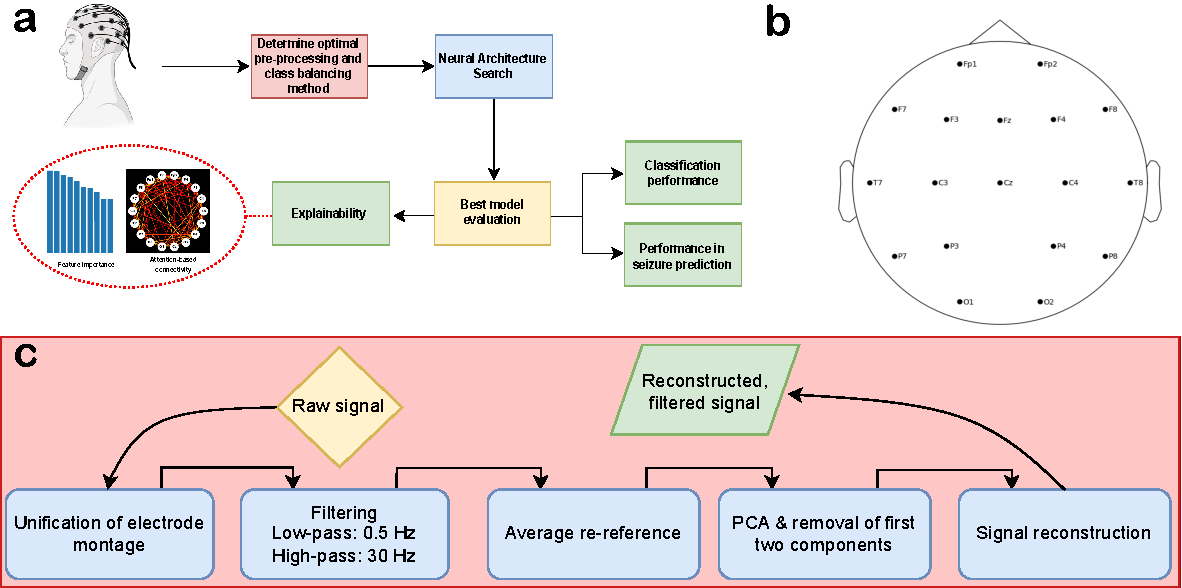
\includegraphics[width=\linewidth]{figures/Fig1.pdf}
    \caption{\textbf{Schematics of the automatic workflow discussed.} \textbf{a} First, for training the \textit{in-silico} system, we represent preprocessed EEG recordings as graphs. Class balancing methods are put in place to prevent wrongful evaluations. Next, this knowledge is then incorporated into the neural architecture search procedure, which automatically finds the best model based on multiple performance evaluation metrics and tests. Importantly, the workflow incorporates an explainability module that returns information on the graph processing and between the input-output relationships. \textbf{b} The positioning of the electrodes used in our computational experiments follows the international 10-20 layout. The anatomical labels correspond to the front (F), parietal (P), pre-frontal (Fp), occipital (O), temporal (T), and central line of the brain (C) \textbf{c} The raw data collected using the set of electrodes in \textbf{b}, enters a preprocessing pipeline with the flow outlined. The clean EEG signals are then fit into the best model found in \textbf{a} to deliver precise, and personalized feedback to the practitioner.}
    \label{fig:graphical_abstract}
\end{figure*}

Finally, during the visual inspection of the pre-processed data, some artefactual activity was still present, manifesting mostly in periods of supra-physiological amplitude peaks of varying lengths. Consequently, we standardized the data using robust standard scaling. This approach allows one to properly standardize the data containing outliers by using the median instead of the mean and interquartile range between the 75th and 25th percentiles. Being a better description of the baseline, these parameters were extracted from the interictal period instead of the preictal one. This pipeline was previously deemed as optimal by an earlier study \cite{MazurekPreprocessing} (see Appendices for further details).

\subsection{Learning EEG representations with graph neural networks}
\color{black} % Temporary solution
A graph constitutes a non-Euclidean geometric space where complex relationships between data points can be embedded and forwarded as inputs into a graph neural network (GNN) \cite{BronsteinGeometricDL}. More formally, a graph $\mathcal{G} = (\mathcal{V}, \mathcal{E})$ is defined as a set of nodes $\mathcal{V} = \{1, \ldots, n\}$ and a set of edges $\mathcal{E} = \{(i,j) \ | \  i,j \in \mathcal{V}\}$ where $(i,j)$ represents a link or interaction between the $i$-th and $j$-th nodes. Initially, each node $i \in \mathcal{V}$ is associated with a column feature vector $\mathbf{h}_{i}^{(0)} \in \mathbb{R}^{d^{(0)}}$. Then, every layer \( l \) of a GNN updates the hidden representation of each node by aggregating information from its neighbors as follows:

\begin{equation} \label{eq:layer}
    \mathbf{h}_{i}^{(l+1)} = f_{\theta} \left( \mathbf{h}_i^{(l)}, \textsc{F} \left( \{ \mathbf{h}^{(l)}_j \, | \, j \in \mathcal{N}_i \} \right) \right),
\end{equation}

where \( \mathbf{h}_{i}^{(l+1)} \) represents the new node representations, \( \mathcal{N}_i \) is the neighborhood of the \( i \)-th node, \( f_{\theta} \) denotes a nonlinearity, and \(\textsc{F}\) is a permutation-invariant aggregator. The choice of the aggregation operator influences the network's expressive power, interpretability, stability, and scalability. We used the GATv2 attentional mechanism to score the relevance of each edge for the final prediction \cite{brody2021gatv2}. Each layer contained a total of $N_K^{(l)}$ attention heads, which we averaged to produce the final representation to be fed into the $(l+1)$-th layer. 

To create the EEG networks, for each subject $s=1,\ldots,24$, window $w=1,\ldots,N_{sw}$, and channel $i=1,\ldots,18$ we created a set of time series $r_{swi}(t)$. Each window $w$, containing a set of 18 aligned time series of length 6 seconds, was labeled as an ictal, preictal, or interictal sample. Edges between channels were constructed by computing the phase locking value (PLV) between each pair of samples \cite{bruna2018plv}. That is,

\begin{equation}
    (i,j)_{sw} =  
    \begin{cases}
        1 \text{  if  PLV}(r_{swi}(t), r_{swj}(t)) > \epsilon_{sw} \\
        0 \text{  otherwise  },
    \end{cases}
    \label{edges}
\end{equation} where

\begin{equation}
    \epsilon_{sw} = \frac{1}{324} \sum_{i=1}^{18}\sum_{j=1}^{18} \text{PLV}(r_{swi}(t), r_{swj}(t))
\end{equation}

is the mean PLV between samples and 324 is the total number of possible edges in a given graph. In the context of seizure detection, both PLV-based edge creation and extraction of handcrafted features capturing spectral properties of the data have proven effective \cite{wang2023plvgraphs,JiaEfficientGraphConv, wijayanto2019fdepilepsy}. As node features, for each sample, we extracted Hjorth parameters, Higuchi and Katz fractal dimensions, line length, and energy of delta (0.5-4 Hz), theta (4-8 Hz), alpha (8-12 Hz), and beta (12-29 Hz) bands. These constituted the components of the feature vectors $\textbf{h}_{swi}^{(0)}$ in Eq. \ref{eq:layer}. We refer to this set of features as Handcrafted Features (HF). For the precise mathematical details applicable to this subsection, we refer the reader to the appendices.

\subsection{Neural architecture search}

Neural architecture search (NAS) aims to automatically find the optimal neural network architecture to solve a given problem. It involves evaluating various numbers of layers, activation functions, and hyperparameters within a computation budget to achieve the best performance as measured by a chosen metric \cite{white2023neural}. Popular NAS methods include evolutionary algorithms, reinforcement learning, Monte Carlo trees, and Bayesian optimization \cite{white2023neural}. In Bayesian architecture search, a surrogate model approximates the objective function to be optimized:
\begin{equation} \label{NAS_surrogate}
    P(m|a) =  \frac{P(a|m)P(m)}{P(a)}
\end{equation}
where $a$ is a given architecture configuration, and $m$ is the performance metric score. This model guides the search by selecting the next architecture $a'$ based on the expected improvement (EI) of the mean loss value across test folds. The improvement $I(a)$ is defined for the minimization problem as:
\begin{equation}
    I(a) = \text{min }(f(a) - f(a^{best}),0) = \text{min }(m - m^{best},0),
\end{equation}
where $f$ evaluates $a$, and $a^{best}$ is the best architecture found so far. The expected improvement is:
\begin{equation}
    EI(a) \doteq \mathbb{E}[I(a)] = \int_{-\infty}^{m_{best}}|I(a)|P(m|a)dm.
\end{equation}
The architecture maximizing $EI(a)$ is evaluated next, and the surrogate model is updated using a Gaussian process, balancing exploration and exploitation to find more optimal architectures \cite{elsken2019neural,white2023neural}.

\subsection{Explainable seizure detection with GNNs}
We assessed edge importance by directly averaging the attention scores of all $N_K^{(l)}$ heads in a given layer. Recall that each attention score is learned during the training procedure and later evaluated using the testing samples. Only samples that were correctly classified were averaged to produce the attention maps. Feature importance identifies subgraphs $\mathcal{G}_{S} \in \mathcal{G}$ and associated features that maximize the mutual information (MI) between the predictions $Y$, the subgraphs $\mathcal{G}_S$, and the masked features $\mathcal{H}_{S}^\mathcal{F} = \mathcal{H}_{S} \odot \mathcal{F}$. $\mathcal{F}$ is a learned binary mask containing the explanability scores for every sample. We obtained the by averaging within classes. 

\subsection{Experiments}
The model was trained to classify data into three categories: preictal, interictal, and ictal, by minimizing the cross-entropy loss function. To evaluate performance, we used stratified cross-validation instead of the leave-one-out (LOO) method used in \cite{MazurekPreprocessing}, which showed significant variability due to patient-specific differences in activity patterns. Some of these patterns included ictal samples with reduced rather than amplified amplitude EEG signals.

Given the relatively small dataset, stratified cross-validation ensured a consistent class distribution and balanced patient representation in both training and testing subsets. All models during the NAS procedure were trained for up to 100 epochs, with early stopping triggered if the validation loss did not improve over 10 epochs. The AdamW optimizer \cite{LoshchilovAdam} was used, with learning rate and weight decay determined via NAS, and a mini-batch size of 1024.

\subsection{Computational resources and software}
The network was implemented in Python 3.10, using the Pytorch 1.13.1 \cite{PaszkeTorch}, Pytorch Geometric 2.2, and Lightning 2.0.4 \cite{falcon2019lightning} libraries \cite{FeyPytorchGeometric} for graph data processing, network construction, and explainability analysis.

Every experiment regarding the model's training was run using 24 AMD EPYC 7742 64-core CPUs, 40 GB of RAM, and 1 Nvidia A100 GPU with 40 GB of RAM in the Athena supercomputer cluster. Explainability metrics were computed using an HP Elite Dragonfly G2 notebook with 8 Intel Core i7-1185G7 CPUs, 32 GB of RAM, and a Mesa Intel Xe Graphics processor.

\section{Results}
\subsection{Neural architecture search}

The main objective of the search was to determine the optimal model architecture. Besides that, we also wanted to evaluate the effectiveness of feature extraction. We ran two searches, one using the proposed HF as node features and the second one using power spectral density (PSD) of the channel signals, following the practice found in \cite{MazurekPreprocessing}.

For each search, the parameters allowed to vary are in Table \ref{tab:nas-params}. The objective of the search was to minimize the average loss across 5 stratified CV folds used to evaluate every run in the search. The search was manually stopped when no further progress was observed, resulting in 102 and 103 runs for the NAS using power spectral density and HF respectively. For HF as node features, the NAS was able to find architectures that resulted in higher mean AUROC values than the ones found for PSD as node features. Based on these findings, we decided to choose the architecture resulting in the highest mean AUROC using HF features (Fig. \ref{fig:final-network}).

\begin{table}[H]
\centering
\begin{tabular}{l||c}
\textbf{Parameter} & \textbf{Range}  \\
\hline
Number of GATv2 layers & 1 to 4  \\
Number of attention head in GATv2 layer & 1 to 10 \\
Final graph pooling & \{max, mean, add\} \\
GATv2 activation function & \{LeakyRELU, ReLU\}  \\
Attention LeakyReLU's slope & $\langle 10^{-3}, 10^{-2} \rangle$ \\
Dropout value & 0.1 to 0.5, interval of 0.1 \\
Learning rate & $\langle10^{-4}, 10^{-2} \rangle$ \\
Weight decay rate & $\langle10^{-4}, 10^{-2} \rangle$ \\
\end{tabular}
\caption{Parameters and ranges sampled during Bayesian NAS.}
\label{tab:nas-params}
\end{table}

\begin{figure}
    \centering
    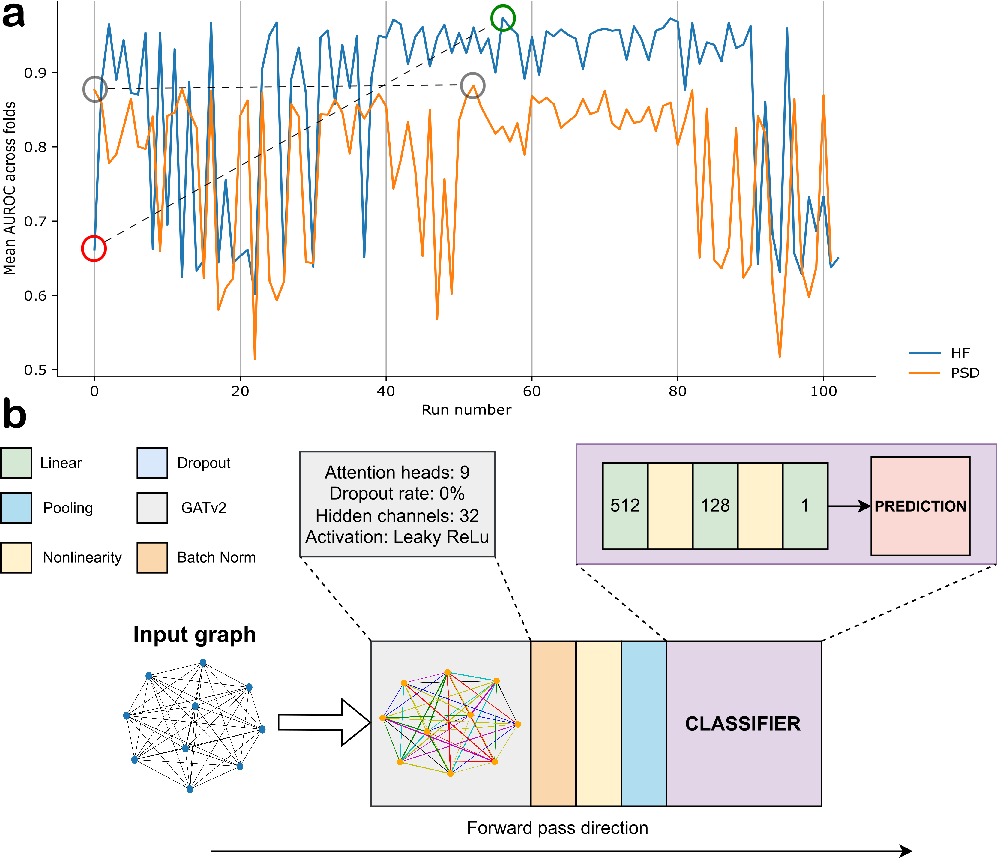
\includegraphics[width=\linewidth]{figures/Fig2.pdf}
    \caption{\textbf{Results of the NAS procedure.} \textbf{a} Mean AUROC across folds for each NAS search iteration using either Handcrafted Features (HF) or Power Spectral Density (PSD) as node features. The red circle marks the starting AUC while the green marks the highest AUC delivered by the NAS. The same for the gray circles using PSD features. \textbf{b} Best performing architecture selected by NAS procedure. Numbers in the blocks denote the number of neurons for each fully-connected layer. We outline the initial architecture in the appendices.}
    \label{fig:final-network}
\end{figure}

\subsection{Final model evaluation}
To further check the results of NAS, we performed an extended evaluation of the final model. We trained the network in Fig. \ref{fig:final-network}b from scratch, using 10-fold cross-validation, obeying the same stratification and normalization principles as for the previous NAS experiments. For each test subset, we computed the AUROC, Sensitivity, Specificity, and Balanced Accuracy. We also compared the models against established machine learning (ML) algorithms: logistic regression (LR), support vector machine (SVM), random forest (RF), and XGBoost (XGB). We trained them using the same cross-validation approach described in the Methods. The average metric values across all folds for the models are shown in Tab. \ref{tab:final-run}. Also, the confusion matrix is shown in \ref{fig:results-final}a for the proposed model. 


The model was able to properly separate the classes, indicated by an average AUROC of 0.9785. Specificity is also consistently reaching high values across all folds, with a mean value of 94.01\%. Sensitivity shows slightly lower performance with a mean value of 89.82\%. Looking into the confusion matrix, we can see that the model is the most robust in the detection of seizure patterns, incorrectly classifying only 3.46\% of the samples present in all folds. The number of errors grows for interictal and preictal classes, as the two are often mistaken with each other by the model. 8.97\% of preictal samples are classified as interictal, and 12.06\% of the interictal were mistaken with preictal class.

Interestingly, classical ML also showed very high performance. SVM, RF, and XGB performed closely to the proposed model, with XGB slightly exceeding its performance. This is surprising, as those models did not take into account the electrode placement, thus omitting any spatial information. It points towards the robustness of using HF as node features for model training, as they proved to be descriptive enough for training a wide range of ML models.


\begin{table}[h]
\centering
\resizebox{\columnwidth}{!}{%
\begin{tabular}{l||ccccc}
\textbf{Model} & \textbf{AUROC} & \textbf{Sensitivity} & \textbf{Specificity} & \textbf{Balanced Acc.} \\
\hline
LR & 0.8061 $\pm$ 0.0021 & 65.63 $\pm$ 0.41 & 82.82 $\pm$ 0.21 & 67.14 $\pm$ 0.37 \\
SVM & 0.9993 $\pm$ 0.0001 & 97.56 $\pm$ 0.11 & 98.78 $\pm$ 0.05 & 90.44 $\pm$ 0.29 \\
RF & 0.9296 $\pm$ 0.0019 & 80.25 $\pm$ 0.39 & 90.12 $\pm$ 0.20 & 73.21 $\pm$ 0.43 \\
XGB & 0.9888 $\pm$ 0.0006 & 92.96 $\pm$ 0.16 & 96.48 $\pm$ 0.08 & 93.36 $\pm$ 0.24 \\
\textit{GATv2}* & 0.9785 $\pm$ 0.0050 & 89.82 $\pm$ 1.51 & 94.91 $\pm$ 0.75 & 92.10 $\pm$ 0.99 \\
\end{tabular}%
}
\caption{Performance of the proposed model (*) compared with other machine learning algorithms. LR, SVM, RF, and XGB stand for Logistic Regression, Support Vector Machine, Random Forest, and XGBoost, respectively.}
\label{tab:final-run}
\end{table}

\begin{figure*}
    \centering
    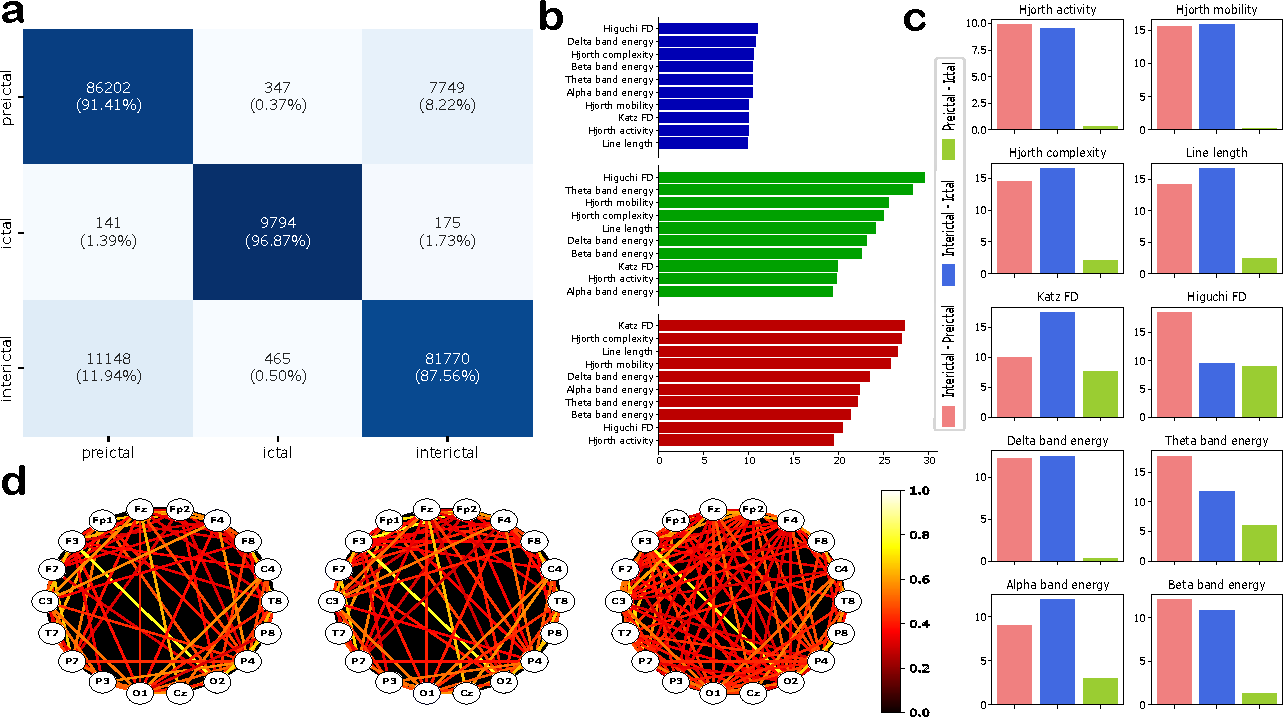
\includegraphics[width=\linewidth]{figures/Fig3.pdf}
    \caption{\textbf{Classification and explainability results of the final model using a preictal window of 10 minutes.} \textbf{a} Confusion matrix for predictions made across all folds. Rows refer to ground truth labels, while columns to predicted ones. Percentage values indicate the number of samples classified to a given class relative to the total number of ground truth samples in that class. \textbf{b} Feature importance for each class obtained from correctly classified samples. Interictal samples in blue, preictal samples in green, and ictal samples in red. Scores are in arbitrary units. \textbf{c} Differences in importance scores between classes in \textbf{b}. \textbf{d} Average edge importance scores obtained from the testing samples across all folds. Edges with attention scores below 0.2 are not shown for clarity. Self-loops are not visualized. Left: interictal class; center: preictal class; right: ictal class.}
    \label{fig:results-final}
\end{figure*}

\subsection{Predictions explainability}
The predictions of the final model were also evaluated in terms of explainability using previously described algorithms. The feature importances are visible in Fig. \ref{fig:results-final}b-c. The scores indicate that for the interictal period, the Higuchi FD, Hjorth complexity, and $\beta$ band energy are the top three distinctive features, with Hjorth mobility and $\delta$ band energy being nearly equally relevant. In the case of preictal windows, we observe an increase in the relevance of line length, which became the second most relevant feature for the classification. Major changes can be seen when making a classification of the ictal periods. Line length, along with Katz FD is shown to be the most relevant, with other features losing their influence. Finally, the changes in functional connectivity based on learned attention coefficients are shown in Fig. \ref{fig:results-final}d. 

\subsection{Performance after increased distance to seizure}
As a final experiment to test the robustness of the model found through NAS, we increased the time-to-seizure used to extract preictal samples. We expected that samples farther from seizure onset would challenge the model's accuracy. Surprisingly, the model maintained high performance, with accuracies above 90\% (see Table \ref{tab:preds-horizon}). Only a slight drop in balanced accuracy occurred when distinguishing samples 60 minutes before seizure onset. This suggests that temporal, frequency, and graph features consistently predict and explain EEG activity leading to seizures. Importantly, feature and edge explainability remained stable across different time horizons (see Appendices).

\begin{table}[!h]
\centering
\resizebox{\columnwidth}{!}{%
\begin{tabular}{l||ccccc}
\textbf{Horizon} & \textbf{AUROC} & \textbf{Sensitivity} & \textbf{Specificity} & \textbf{Balanced Acc.} \\
\hline
10 (min) & 0.9785 $\pm$ 0.0050 & 89.82 $\pm$ 1.51 & 94.91 $\pm$ 0.75 & 92.10 $\pm$ 0.99 \\
20 (min) & 0.977 $\pm$ 0.005 & 89.4 $\pm$ 1.3 & 94.7 $\pm$ 0.7 & 92.1 $\pm$ 0.9 \\
30 (min) & 0.976 $\pm$ 0.004 & 89.2 $\pm$ 1.1 & 94.6 $\pm$ 0.6 & 91.9 $\pm$ 0.7 \\
60 (min) & 0.9721 $\pm$ 0.0073 & 88.3 $\pm$ 1.9 & 94.1 $\pm$ 0.9 & 91.3 $\pm$ 1.3 \\
\end{tabular}%
}
\caption{Performance of \textit{GATv2} in Tab. \ref{tab:final-run} as a function of the temporal horizon used to define samples as preictal.}
\label{tab:preds-horizon}
\end{table}

\subsection{Predictive capabilities of a well-trained classifier}
Lastly, we decided to evaluate the capability of the classifiers trained on data including different preictal horizons to perform proxy seizure prediction. An accurate seizure detection pipeline does not guarantee reliable prediction of the time until the next pathological activity. Predicting seizures based on short time windows is challenging, even for clinicians. We therefore look at this problem from the preictal activity classification perspective. Conceptually, if the model can accurately predict preictal activity, it follows that the preictal prediction is indicative of the incoming seizure.

Thus, we construct the following experiment: for each of the tested preictal horizons separately, we extract preictal test samples from each fold along with the information if the model correctly classified them as preictal during testing. Then, we determine how far in time was the given preictal sample from the beginning of the seizure. We plot the accuracy of the model in classifying preictal samples depending on the samples' proximity to the beginning of the ictal activity.

Our model maintained over 85\% accuracy in detecting preictal activity up to 60 minutes before onset, with slight decreases for the samples coming from the 40-60 minutes range (Fig. \ref{fig:predictive-horizon}; see also Appendices). This follows the common expectations that such classification should get harder as the proximity to the seizure increases. Interestingly, a similar slight drop is observed for samples close to the seizure. A possible explanation of this phenomenon is the occurrence of signs of pathological activity in those samples as the ictal period nears, making the classification harder.

\begin{figure*}
    \centering
    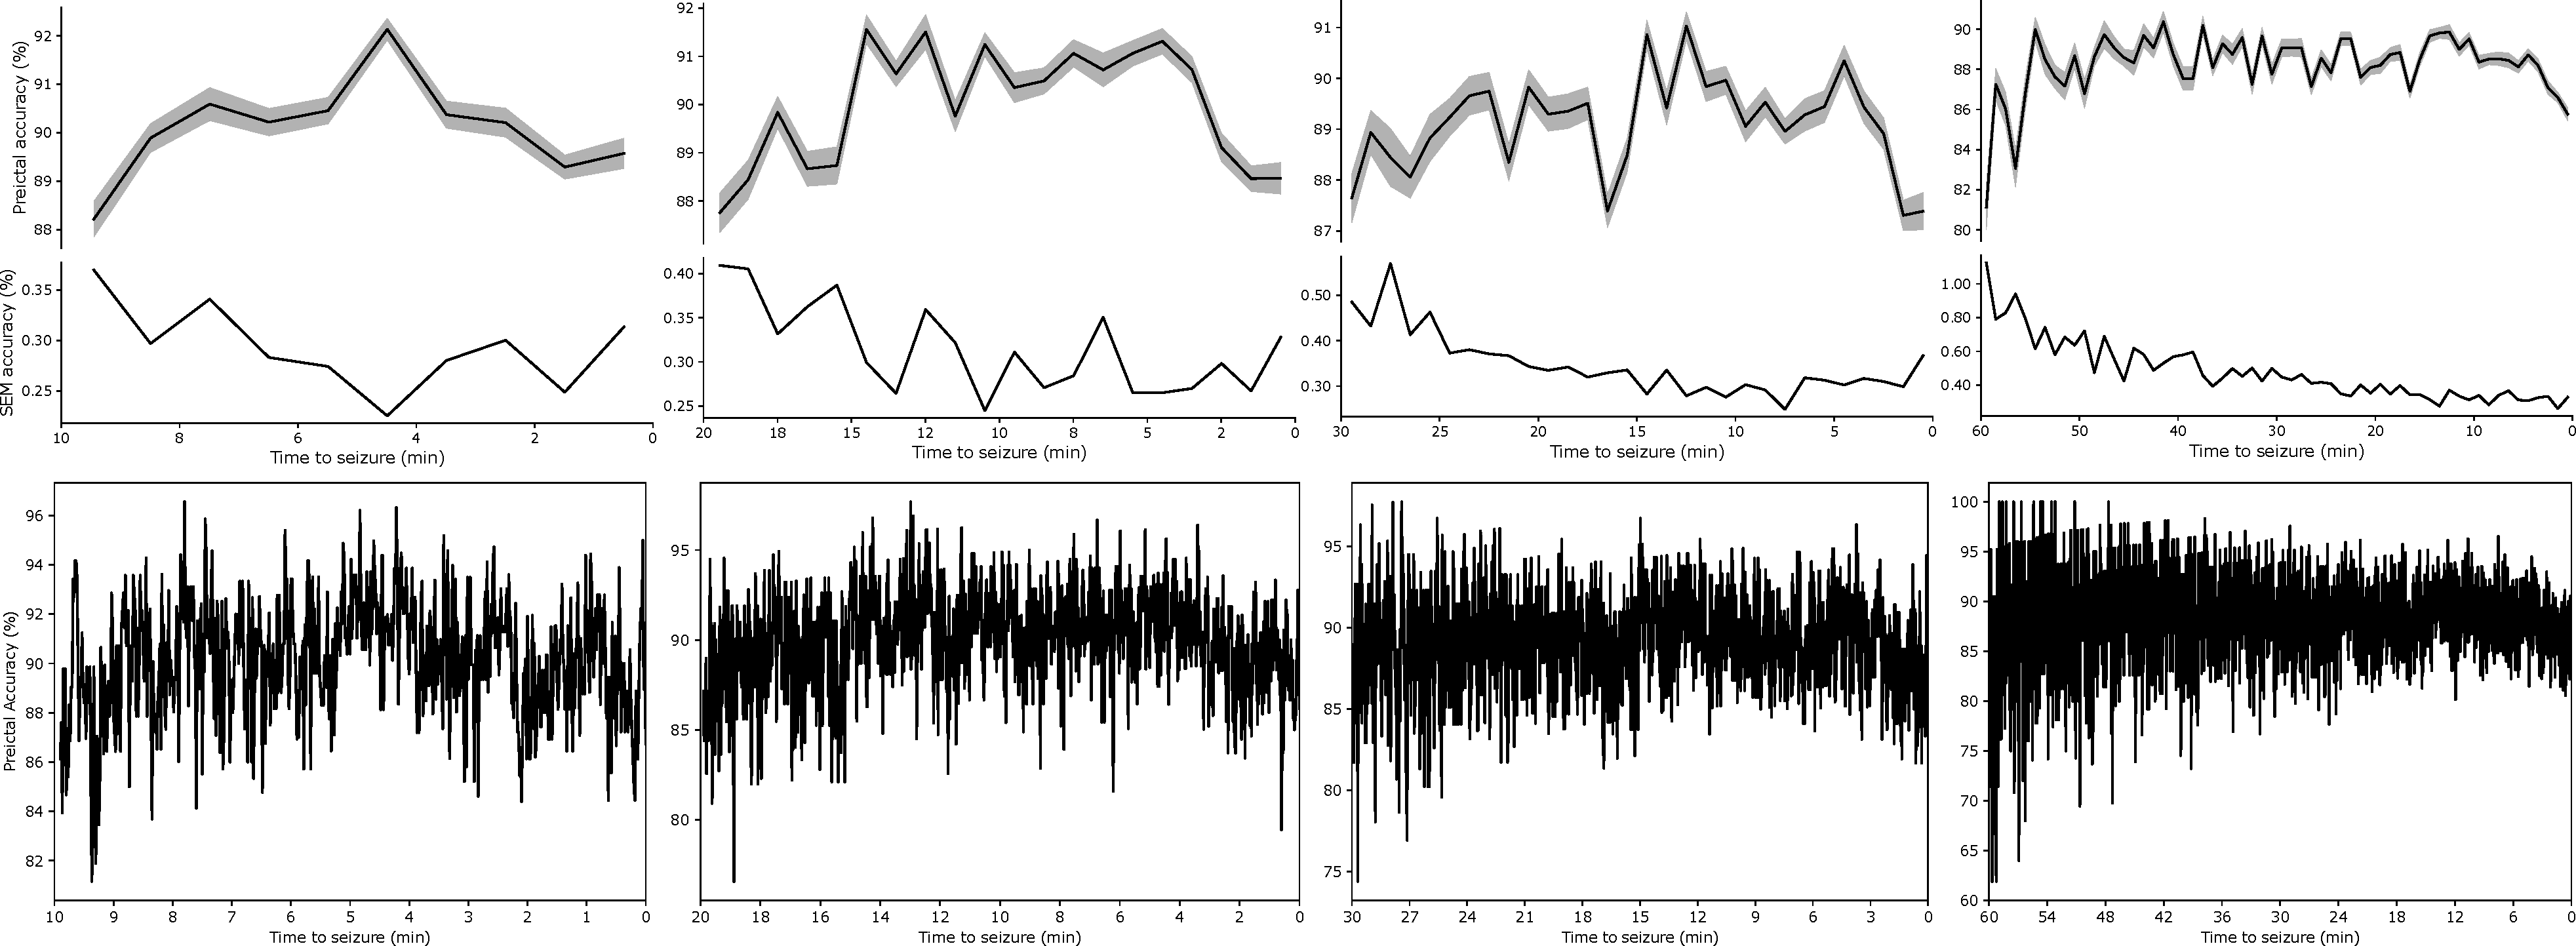
\includegraphics[width=\linewidth]{figures/Fig4.pdf}
    \caption{\textbf{Indirect predictions of seizure onset.} Plots showing the accuracy for the preictal class depending on samples' proximity to seizure. In the top row, plots were obtained by smoothing the original one with a 60-second window, inside which the accuracies were averaged. Shaded regions show 1 standard error of this mean (SEM). In the bottom row, the raw accuracies are displayed.}
    \label{fig:predictive-horizon}
\end{figure*}

\section{Discussion}

In this work, we extensively studied GNN-based epileptic EEG classification. Namely, we aim to classify time windows from EEG recordings into interictal, preictal, and ictal categories. Building on previous work on signal pre-processing \cite{MazurekPreprocessing}, we start with filtering the data and use class balancing methods to mitigate shortcomings of the used dataset. Then, to establish the optimal network architecture, we perform NAS during which we additionally evaluate the effectiveness of proposed HF as node features compared to power spectrum-based ones. We show that NAS led to significant gains in the model's performance, with the approach using the proposed HF performing better than when evaluating only the power spectrum as node features. This provides an important observation for future research, as NAS is generally model-agnostic and can be effectively used to tune parameters, potentially leading to large performance gains. Lastly, we evaluate the obtained model using 10-fold stratified cross-validation and compare its performance against established ML models. Other ML models that were tested also show high performance, possibly indicating that the usage of the proposed combination of HF features is useful in EEG-related tasks. 

\subsubsection*{Automated EEG analyses in pediatric epilepsy}
Multiple works in the last decade have been dedicated to machine learning (ML) methods for pediatric seizure classification \cite{ahmed2022review}, with accuracies ranging from 70\% to 96\% accuracies. The CHB-MIT dataset is predominantly used for such analyses, with a benchmark accuracy of 96\% using an SVM \cite{shoeb2010applications}. Also using the same SVM, accuracy has been increased to 97.74\% when combined with the adequate features \cite{samiee2015features}. Notably, ensemble learning \cite{alotaibi2021ensemble} and and hand-crafted features\cite{khan2012automatic} achieved a 100\% accuracy in detecting ictal samples but, given that these systems were trained and tested on 7 and 10 subjects respectively, we cannot issue a direct comparison. More sophisticated alternatives based on particle swarm optimization achieved competitive but slightly inferior results \cite{kiranyaz2014swarm}, albeit claiming patient specificity. When investigating spectral characteristics, accuracies remained around 75\% \cite{ravish2012automated}. Our results suggest that thorough but automated preprocessing and feature extraction of EEG signals \cite{MazurekPreprocessing} leaves room for improvement (see Table \ref{tab:final-run}). Unfortunately, on preictal classification, there is a lack of research using classical ML methods. Moghim and Corne \cite{moghim2014predicting} examined preictal samples ranging from 1 to 25 minutes before seizure onset, achieving accuracies of 96.13\% and 94.2\%, respectively. In our study, we extended this analysis to preictal samples occurring up to 60 minutes prior to seizures, successfully distinguishing approximately 90\% of these samples with a low error rate in misclassifying interictal activity (Fig. \ref{figs2:confusion_lookbacks}). This sets a promising benchmark for future research in early seizure prediction.

In comparison to existing AI-based methods for seizure detection in pediatric datasets, our proposed solution demonstrates strong performance. The current state of the field rarely integrates the 3 types of EEG samples although having a system able to handle everything at once instead of multiple subsystems dealing with each binary problem would be beneficial for clinical applications (Table \ref{tab:pediatric_AI}). Our model, GATv2, performs competitively with state-of-the-art approaches, achieving an AUROC of 0.9785, a sensitivity of 89.82\%, and a balanced accuracy of 92.10\%. This places it close to high-performing methods but with the added benefit of graph-based learning, which has been shown to excel at capturing complex structural information. Our results also highlight the robustness of GATv2 across different preictal definitions (Table \ref{tab:preds-horizon}), with only marginal drops in performance as the temporal horizon changes.

In contrast to other models that lack explainability, GATv2 has the potential to be integrated with explainable AI methods, a crucial feature for clinical applications. However, while our approach effectively handles complex relationships in data, it still lags slightly behind in raw accuracy compared to purely convolutional or statistical models, which excel in maximizing classification accuracy on seizure detection. Moreover, while we report strong performance across different preictal windows, models like XGBoost maintain higher overall accuracies with simpler architectures. Thus, our method’s strength lies in its adaptability and interpretability, though there may be trade-offs in fine-tuning for peak performance compared to more traditional models. The latter can be addressed by incorporating more extensive NAS procedures aimed at finding the best combination of parameters and architectures to secure stable performances across conditions.

\subsubsection*{Inherent interpretability of GNNs' predictions enhance AI applicability in the medical domain}
Transparency in computational medicine should be a requirement for any model to be trusted. Explainable AI workflows offer an interesting trade-off between increased model capacity, complexity, interpretability, and robustness. Experiments to identify the most relevant node features for each prediction indicate that the Higuchi fractal dimension and Katz fractal dimension are the most descriptive features for preictal and ictal periods respectively. During interictal periods, no single feature proved to be more informative than the others, suggesting that incorporating additional features might enhance class specificity. Additionally, modeling the signal as a graph reveals the complex relationships between electrodes, with weights reflecting their contribution to the model's output. Attention scores from GATv2 layers establish edge importance, offering insights into changes in brain connectivity across different EEG periods. An overall increase in brain-wide functional connectivity from the interictal to the preictal to the ictal period indicates a growing synchronization of cortical activity (Fig. \ref{fig:results-final}d). This is coherent with clinical knowledge, as seizures often spread across the cortex from the source. Also, some regions consistently receive high attention coefficient values, namely O2-F3, P7-F7, and O2-P4-P8. These areas may be related to one or more epileptogenic focuses. Furthermore, albeit requiring more research, these changes in connectivity are potentially useful for distinguishing present and imminent seizure periods. In clinical environments, these changes may serve as valuable features for classification purposes and aid in seizure focus localization, as strongly interconnected regions consistently appear across all sample types, potentially indicating areas responsible for the most pathological activity.

\subsubsection*{Predictive capabilities of well-trained classifiers}
Prediction of the incoming seizure is another crucial task for effective epilepsy management. It is a nontrivial problem, as indicators of incoming seizure are subtle and not consistent across patients.  
A naïve approach to the prediction of future seizures would imply the minimization of a cost function incorporating the time to seizure label – for example, by minimizing the mean squared error between the true and predicted time. However, in our experiments, we try to use the classification model as a proxy predictor by classifying preictal activities. We build on the notion that if the model is able to correctly classify preictal samples, those classifications can be treated as indicators of incoming seizures. Our model shows robust preictal period classification accuracy, even in preictal horizons as long as 1 hour.

For example, in the testing phase, samples could be sequentially forwarded into the classifier, and a posterior belief of the time to seizure given the predicted preictal class could be computed. Formally,
\begin{equation*}
    P(time|preictal) \propto (preictal|time)P(time), 
\end{equation*}
where $time$ is a given time window, $P(time)$ is a prior belief, and $P(preictal|time)$ is the likelihood of predicting preictal activity given an unknown time. The former might take several forms, while the latter could be extracted from the trained model by evaluating the ability of the AI system to maintain accuracies across different horizons (Fig. \ref{fig:predictive-horizon}). Moreover, the posterior belief could be constantly updated to decrease the uncertainty of the model via a Gaussian or partially observable Markov decision processes \cite{kaelbling1998planning}. This simplification needs to be further evaluated and refined. Still, it can apply to any model conditioned to acceptable accuracies in detecting preictal EEG samples. In this aspect, automatic and fast preprocessing of EEG samples, such as the one investigated, represents a key element for this framework to succeed.

\subsubsection*{Future work and study limitations} The dataset contained a relatively small number of subjects compared to those present in cohort studies, potentially limiting its immediate clinical translation. Secondly, a more precise evaluation of the different filtering frequencies and PCA usage could be performed - the frequency threshold and the number of PCA components can be tuned. There are some findings in the literature suggesting that high-frequency oscillations can have diagnostic value in detecting ictal and preictal patterns \cite{jung2019hfoepilepsy} and they should be maintained in the signal. Lastly, the NAS search space can also be expanded by incorporating added architecture parameters (e.g., number of neurons). This would further increment the robustness of the final model w.r.t. unseen samples. 

Although classical machine learning algorithms achieved similar classification performance, our solution offers two key advantages. First, we focused on generating explainable predictions that utilize the complex spatial and temporal structure of EEG signals, which only graph attention networks can accomplish. Second, for clinical deployment, any model must be validated on large, independent datasets — a challenge for classical models like SVMs and decision trees. Therefore, our solution is well-positioned despite requiring ongoing validation with larger datasets. In a clinical setting, combining multiple models could enhance trust in algorithmic decisions. Once validated, the explanations provided by a graph attention classifier can significantly aid in diagnosing epilepsy and may even improve surgical planning.

\subsection*{Conclusions}
We present a comprehensive, end-to-end, and explainable approach for developing graph deep learning models for EEG classification and seizure prediction in epileptic patients. Our approach includes fully automated PCA-based denoising and class imbalance handling methods, which significantly enhance the model’s performance. We then optimize the model’s architecture and training hyperparameters using Bayesian architecture search. Next, we apply explainability algorithms to identify feature and edge importances, offering insights into the decision boundaries learned by the model. Our results demonstrate that the model maintains high performance when classifying samples from up to 60 minutes before a seizure. Lastly, we evaluate the model’s potential to predict seizures by classifying preictal samples, thus advancing the field in two different areas: simultaneous classification of ictal, preictal, and interictal activity while retaining interpretable and explainable results

\printcredits

\section*{Declaration of competing interests}
The authors declare no conflicts of interest.

\section*{Data availability}
The dataset is available at \url{https://physionet.org/content/chbmit/1.0.0/}. The code with the usage instructions is available at \url{https://github.com/szmazurek/sano_eeg}.

\section*{Acknowledgements}
The publication was created within the project of the Minister of Science and Higher Education "Support for the activity of Centers of Excellence established in Poland under Horizon 2020" on the basis of the contract number MEiN/2023/DIR/3796, and has received funding from the European Union’s Horizon 2020 research and innovation programme under grant agreement No 857533. This publication is supported by Sano project carried out within the International Research Agendas programme of the Foundation for Polish Science, co-financed by the European Union under the European Regional Development Fund. We gratefully acknowledge Polish high-performance computing infrastructure PLGrid (HPC Center: ACK Cyfronet AGH) for providing computer facilities and support within computational grant no. PLG/2023/016289.

\appendix

\section{Appendix 1}

In this section, we show complementary results to the main text. Additionally, we provide formal mathematical descriptions of the graph attention layers, the neural architecture search, and spectral features.

\setcounter{equation}{0}
\renewcommand{\theequation}{A.\arabic{equation}}
%\setcounter{section}{0}
%\renewcommand{\thesection}{S\arabic{section}}
\setcounter{figure}{0}
\renewcommand{\thefigure}{A\arabic{figure}}
\setcounter{table}{0}
\renewcommand{\thetable}{A\Roman{table}}

\subsection{Graph neural networks with attention}
GNNs can learn non-trivial representations by leveraging the complex topological organization of the data \cite{velivckovic2023everything,wu2019graphsurvey}. Intuitively, a graph constitutes a non-Euclidean geometric space where complex relationships between data points can be embedded and forwarded as inputs into a GNN \cite{BronsteinGeometricDL}. More formally, a graph $\mathcal{G} = (\mathcal{V}, \mathcal{E})$ is defined as a set of nodes $\mathcal{V} = \{1, \ldots, n\}$ and a set of edges $\mathcal{E} = \{(i,j) \ | \  i,j \in \mathcal{V}\}$ where $(i,j)$ represents a link or interaction between the $i$-th and $j$-th nodes. Initially, each node $i \in \mathcal{V}$ is associated with a column feature vector $\mathbf{h}_{i}^{(0)} \in \mathbb{R}^{d^{(0)}}$.

Every layer $l$ of a GNN updates the hidden representation of each node by aggregating information from the neighborhoods: 
\begin{equation} \label{layer}
    \mathbf{h}_{i}^{(l+1)} = f_{\theta} \left( \mathbf{h}_i^{(l)}, \textsc{F} \left( \{ \mathbf{h}^{(l)}_j \, | \, j \in \mathcal{N}_i \} \right) \right),
\end{equation}
where $\textbf{h}_{i}^{(l+1)} \in \mathbb{R}^{d^{(l+1)}}$ are the new node representations, $\mathcal{N}_i$ is the neighborhood of the $i$-th node, $f_{\theta}$ denotes a nonlinearity, and $\textsc{F}$ is a permutation-invariant aggregator. Several proposals exist for the aggregation operator, determining the expressive power, interpretability, learning stability, and scalability of the network \cite{velivckovic2023everything}. Attentional aggregators offer an interesting trade-off by independently aggregating local information and subsequently scoring the relevance of each edge for the final prediction \cite{velickovic2018graph}. Following \cite{brody2021gatv2}, we computed a scalar score,

\begin{equation} \label{score_e}
    e_{i,j}^{(l)} = \mathbf{a}^{(l)\top}  \cdot \textsc{LeakyReLU}(\mathbf{W}^{(l)} \cdot [\mathbf{h}_{i}^{(l)} || \mathbf{h}_{j}^{(l)}]),
\end{equation} 

where $\mathbf{a}^{(l)} \in \mathbb{R}^{d^{(l+1)}}$ and $\mathbf{W}^{(l)} \in \mathbb{R}^{d^{(l+1)} \times 2d^{(l)}}$ are learned parameters, and $||$ concatenates $\mathbf{h}_{i}^{(l)}$ and $\mathbf{h}_{j}^{(l)}$ along the first axis. These scores are normalized within the neighbors,

\begin{equation} \label{score_alpha}
    \alpha_{ij}^{(l)} = \frac{\exp\left(e_{ij}^{(l)}\right)}{\sum_{k \in N_i\cup\{i\}} \exp\left(e_{ik}^{(l)}\right)},
\end{equation}

where $\alpha_{ij}^{(l)}$ is the final attention score of each edge. Lastly, we computed the new representations learned by the $l$-th layer by weighting the features with the learned attention scores: 

\begin{equation} \label{representation}
    \textbf{h}_{i}^{(l+1)} = f_{\theta}\left( \sum\nolimits_{j \in N_i \cup\{i\}} \alpha_{ij}^{(l)} \mathbf{W}^{(l)} \cdot \mathbf{h}_{j}^{(l)} \right).
\end{equation}
In practice, multiple attention \textit{heads} have been proven to improve the stability of learning \cite{velickovic2018graph,brody2021gatv2}. For each head, an independent attention score $\bm{\alpha}_n^{(l)}$ is learned (i.e., in Eq. (\ref{score_alpha})). Finally, the outputs in Eq. (\ref{representation}) of all $N_K^{(l)}$ heads are concatenated or averaged to give the $l+1$ layer node representation.

\subsection{Feature and edge explanations}
As outlined earlier in the main text, we aimed to explain the network's focus when detecting the presence of an epileptic seizure. We restricted our attempts to provide intuitive explanations of the most important edges and features.

Edge importance can be directly assessed by averaging the attention scores in Eq. (\ref{score_alpha}) over all $N_K^{(l)}$ attention heads in a given layer 

\begin{equation} \label{edge_explain}
    \mathbf{A}^{(l)} = \frac{1}{N_K^{(l)}} \sum_{n=1}^{N_K}  \bm{\alpha}_{n}^{(l)}.
\end{equation}

On the other hand, feature importance aims to identify a subgraph $\mathcal{G}_{S} \in \mathcal{G}$ and associated features $\mathcal{H}_{S} = \{ \mathbf{h}_i \mid i \in \mathcal{V}_{S} \}$ relevant for the GNN predictions \cite{Ying2019GnnX}. A separate \textit{explainer} model is optimized to maximize the mutual information $MI$ between the predicted labels $Y$ and the selected subgraph and features $(\mathcal{G}_S,\mathcal{H}_S)$: 

\begin{equation}\label{mutual_info}
    \max_{\mathcal{G}_{S}, \mathcal{F}} MI(Y, (\mathcal{G}_{S}, \mathcal{F})) = H(Y) - H(Y \mid \mathcal{G}_{S}, \mathcal{H}_{S}^\mathcal{F}),
\end{equation}
where $H(\cdot)$ is the Shannon entropy, $\mathcal{H}_{S}^\mathcal{F} = \mathcal{H}_{S} \odot \mathcal{F}$ is a subset of masked features, and $\mathcal{F}$ is a learned binary mask identifying the most informative features of the selected subgraph.
The feature explainability scores $\mathcal{F}$ were obtained for every sample and later averaged for every class. 

\subsection{Neural architecture search}
Neural architecture search (NAS) is a process of automatically finding the optimal architecture of a neural network to solve a given problem. The architecture of the network can be viewed as a composition of various layers of neurons, connections between them, and hyperparameters defining their properties. The process is initialized with a single architectural instance $A$ which is later left free to evolve to find the combination of free parameters that produce the best outcomes. The initial choice of parameters can be seen in Fig. \ref{figs1:initial-architecture}.

\begin{figure}[h]
    \centering
    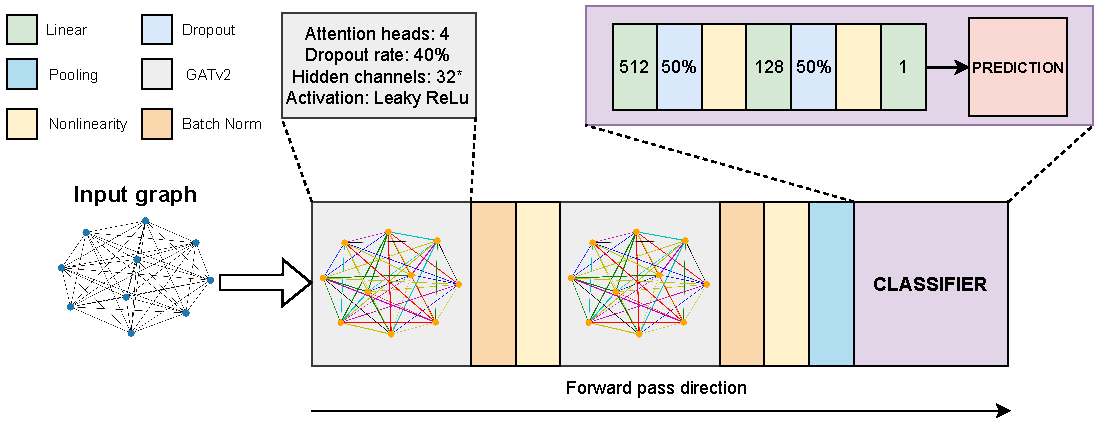
\includegraphics[width=\linewidth]{figures/FigS1.pdf}
    \caption{\textbf{Initial architecture in the NAS procedure.} Numbers in the blocks denote the number of neurons for each fully-connected layer.}
    \label{figs1:initial-architecture}
\end{figure}

\subsection{Detailed description of extracted node features}
\label{chapter:appendix-2}
\subsubsection{Fast Fourier Transform}
For the experiments to determine optimal pre-processing, the time series were transformed into a vector representing power spectral density:
\begin{equation}
    S_k= |X_k|^{2},
\end{equation}
where $S(f_k)$ is a power spectral density at frequency $f_k$ and $X(f_k)$ is a value of
Fourier coefficient at frequency $f_k$. Fourier coefficients are obtained by applying the Discrete Fourier Transform (DFT) to the input signal x(t). The kth coefficient is obtained by:
\begin{equation}
    X_k = \sum_{i=0}^{N-1}x_i e^{-ki\frac{2\pi j}{N}}, k \in {0,1,2, ..., N-1},
\end{equation}
where $N$ is the length of the sample, $N$ is the sample length, $e$ is an Eurler's number and $j$ is the imaginary number.
The DFT was computed using the Fast-Fourier Transform (FFT) algorithm introduced by \cite{Cooley1965FFT} and
implemented in the Python library Numpy 1.25.2 \cite{harris2020numpy}. Noteworthy, in the case of this paper the coefficients obtained with DFT were normalized with $N$.
\subsubsection{Phase Locking Value}
The Phase Locking Value (PLV) \cite{bruna2018plv} is a measure used when constructing adjacency matrices for the samples in architecture search experiments. PLV between two signals $i$ and $j$ is defined as:
\begin{equation}
    PLV_{i,j} = \frac{1}{N}|\sum_{n=1}^{N}{e^{-j(\phi_i(n)-\phi_j(n))}}|,
\end{equation}
where $\phi(n)$ is the instantaneous phase of each signal at timestep $n$.
\subsubsection{Hjorth Parameters}
Hjorth parameters \cite{hjorth1970params} are indicators of statistical properties of the analyzed time series. Activity, which is denoted simply as a variance of the observed time series:
\begin{equation}
    A(x(t)) = var(x(t)).
\end{equation}
It allows us to measure if the high-frequency components occur often in the signal.
Mobility, expressed as:
\begin{equation}
    Mob(x(t)) = \sqrt{\frac{A(x'(t))}{A(x(t))}},
\end{equation}
shows the mean frequency. Lastly, Complexity is expressed as:
\begin{equation}
    Compl(x(t))=\frac{Mob(x'(t))}{Mob(x(t))},
\end{equation}.
This measure shows the similarity of the measured signal to the pure sine wave.
\subsubsection{Line length}
Line length is calculated as a normalized running sum of the absolute differences between consecutive signal samples within a chosen time window, providing a measure of signal variability \cite{esteller2001linelength}. It is expressed as:
\begin{equation}
    L(x(t))= \sum_{i=1}^{N-1}(|x_{i+1} - x_{i}|),
\end{equation}
where $N$ is the number of samples in a time window. In our experiments, we use a normalized version, which is simply dividing the obtained line length by the number of samples in the window $L_n(x(t)) = \frac{1}{N-1}L(x(t))$.

\subsubsection{Fractal dimensions}
Intuitively, the fractal dimension (FD) of a time series can be understood as a measure of the deviation of a signal from a 1D straight line towards a 2D plane covering the entire analyzed time window domain \cite{higuchi1988fd,esteller2001katzfd}.
Katz FD of a signal can be denoted as:
\begin{equation}
    D_{Katz}(x(t)) = \frac{\log_{10}(N)}{\log_{10}(\frac{d}{L(x(t))})+\log_{10}(N)},
\end{equation}
where $d$ is a \textit{diameter} defined as the distance from the first point in the analyzed time window and the one that leads to maximization of the distance:
\begin{equation}
    d = max_{t \in N, t\neq{t_1}}|x(t_1) - x(t)|
\end{equation}

\subsubsection{Signal energy}

The energy of a discrete-time signal of length N is defined as:
\begin{equation}
    E(x(t)) = \sum_{n=0}^{N}x(t_n)^{2} 
\end{equation}
In this work, we calculated the energy of a given time series associated with an EEG channel for different energy bands by first applying the 4th-order Butterworth filter to include only the analyzed frequency band. The frequency bands were defined as follows: delta (0.5 to 4 Hz), theta (4 to 8 Hz), alpha (8 to 13 Hz) and beta (13 to 29 Hz). The lower limit of the delta band and the upper one of the beta band were chosen to fall within the filtering band ranges (0.5 to 30 Hz) obtained in the pre-processing step.

\subsection{Alternative preprocessing pipelines}
At first, the proposed pre-processing method was tested against two cases - no pre-processing and band-pass filtering between 0.5 Hz and 30 Hz extended additionally with average re-referencing. The results are visible in Tab. \ref{tab:pre-processing}. The proposed method significantly improved the tested model's ability to discriminate between preictal and ictal periods compared to using only raw signals or pre-processed ones without any additional artifact removal algorithm. During these experiments, no class imbalance handling methods were used yet.
\begin{table}[H]
\centering
\begin{tabular}{l||c}

\textbf{Pre-processing method} &  \textbf{Average AUROC} \\
\hline
None & $0.7872 \pm 0.1941$ \\
Filtering and re-reference & $0.8069 \pm 0.1891$ \\
Our protocol & $\mathbf{0.8754 \pm 0.1366}$ \\
\end{tabular}
\caption{Performance of the model using different data pre-processing methods. Bold numbers indicate the best results.}\label{tab:pre-processing}
\end{table}

Next, we proceeded to evaluate the methods for class imbalance handling. For these experiments, we used the data pre-processed with the method that showed superior performance in the previous trials. We tested various combinations of previously described balancing methods, applying them to different classes and data subsets. The results are shown in Tab. \ref{tab:balancing-results}. We observed only minor improvements in performance compared to the preprocessing-only baseline. The best results were observed for using window overlap for all classes, increasing the average AUROC by 0.0165. Combining this method with class weights resulted in nearly identical performance. Noteworthy, some methods led to a drop in performance compared to the baseline. It was especially prevalent in the experiment where window overlap was used along with SMOTE on the training subset samples. The mean AUROC dropped to 0.8101 from the baseline of 0.8754. This possibly indicates that the straightforward application of SMOTE to the channel's time series led to the creation of unrepresentative samples, which resulted in a performance drop. This problem requires further evaluation, which we leave for future work. These results are better detailed in previous work from the team \cite{MazurekPreprocessing}.

\begin{table}[H]
\centering
\begin{tabular}{l||c}

\textbf{Method} & \textbf{Average AUROC} \\
\hline
Undersampling & $0.8639 \pm 0.1614$ \\
Window overlap (ictal samples only) & $0.8851 \pm 0.1497$ \\
Window overlap (all samples) & $\mathbf{0.8919 \pm 0.1217}$ \\
Window overlap (all samples) + undersampling & $0.8858 \pm 0.1556$ \\
Positive class weight & $0.876 \pm 0.1486$ \\
Window overlap (ictal samples only) + positive class weight & $0.8845 \pm 0.1512$ \\
Window overlap (all samples) + positive class weight & $\mathbf{0.8919 \pm 0.1375}$ \\
Window overlap (all samples) + SMOTE  (training set and LOO patient) & $0.8793 \pm 0.1314$ \\
Window overlap (all samples) + SMOTE  (training set) & $0.8101 \pm 0.1616$ \\
Window overlap (all samples) + SMOTE (LOO patient) & $0.8506 \pm 0.1851$ \\
Window overlap (all samples) + SMOTE (LOO patient) + positive class weight & $0.8474 \pm 0.2005$ \\

\end{tabular}
\caption{Performance of the model using different class imbalance handling methods. Bold numbers indicate the best results.}\label{tab:balancing-results}
\end{table}

\subsection{Robustness w.r.t. the predictive horizon}

We performed additional evaluations of the models trained for different preictal lookback horizons. The results are shown in Tables \ref{tab:numbers_1200}, \ref{tab:numbers_1800}, and \ref{tab:numbers_3600}; and figures \ref{figs2:confusion_lookbacks}. Metric values show that the model can maintain its performance with increasing preictal lookback. These results are promising, as they indicate that the model found by the NAS was not overturned to perform only on a certain data subset. It also shows the potential usefulness of the model in seizure prediction tasks with long predictive horizons. Similar things can be seen examining the confusion matrices, as the performance for given classes did not change significantly between the horizons. It is visible that the model maintained a seizure detection perspective, where the number of samples stays roughly the same, whereas, for the remaining classes, it grows significantly. 

\begin{table}[h]
    \centering
    \begin{tabular}{c|c|c|c|c}    
        AUROC & F1-score & Sensitivity & Specificity & Accuracy \\
        \hline
        \hline
        0.9763 & 89.14 & 89.14 & 94.57 & 92.03 \\
        0.9731 & 88.33 & 88.33 & 94.17 & 91.32 \\
        0.9769 & 89.59 & 89.59 & 94.79 & 92.04 \\
        0.9766 & 89.32 & 89.32 & 94.66 & 91.78 \\
        0.9775 & 89.44 & 89.44 & 94.72 & 92.0 \\
        0.9841 & 91.57 & 91.57 & 95.78 & 93.68 \\
        0.9814 & 90.43 & 90.43 & 95.21 & 92.46 \\
        0.9669 & 86.77 & 86.77 & 93.39 & 90.11 \\
        0.9826 & 90.96 & 90.96 & 95.48 & 93.05 \\
        0.9759 & 89.04 & 89.04 & 94.52 & 92.02 \\
        \hline
        0.977 (0.005) & 89.4 (1.3) & 89.4 (1.3) & 94.7 (0.7) & 92.1 (0.9) \\
        \hline
    \end{tabular}
\caption{Metrics describing the performance of the final model on the test sets from consecutive folds using a preictal window of 20 minutes. All metrics except AUROC are denoted in percentages. Accuracy was calculated using the balanced version. The last row describes the mean for a given metric and its standard deviation - between parenthesis.}
\label{tab:numbers_1200}
\end{table}

\begin{table}[h]
    \centering
    \begin{tabular}{c|c|c|c|c}    
        AUROC & F1-score & Sensitivity & Specificity & Accuracy \\
        \hline
        \hline
        0.9768 & 89.3 & 89.3 & 94.65 & 91.94 \\
        0.9774 & 89.51 & 89.51 & 94.76 & 92.11 \\
        0.9774 & 89.44 & 89.44 & 94.72 & 91.96 \\
        0.9819 & 90.59 & 90.59 & 95.29 & 92.91 \\
        0.9695 & 87.52 & 87.52 & 93.76 & 90.65 \\
        0.9819 & 90.92 & 90.92 & 95.46 & 92.75 \\
        0.9743 & 88.83 & 88.83 & 94.42 & 91.73 \\
        0.9719 & 87.95 & 87.95 & 93.98 & 91.31 \\
        0.976 & 89.18 & 89.18 & 94.59 & 91.91 \\
        0.9729 & 88.29 & 88.29 & 94.15 & 91.35 \\
        \hline
        0.976 (0.004) & 89.2 (1.1) & 89.2 (1.1) & 94.6 (0.6) & 91.9 (0.7) \\
        \hline
    \end{tabular}
\caption{Metrics describing the performance of the final model on the test sets from consecutive folds using a preictal window of 30 minutes. All metrics except AUROC are denoted in percentages. Accuracy was calculated using the balanced version. The last row describes the mean for a given metric and its standard deviation - between parenthesis.}
\label{tab:numbers_1800}
\end{table}

\begin{table}[h]
    \centering
    \begin{tabular}{c|c|c|c|c}    
        AUROC & F1-score & Sensitivity & Specificity & Accuracy \\
        \hline
        \hline
        0.975 & 89.09 & 89.09 & 94.54 & 92.03 \\
        0.9738 & 88.72 & 88.72 & 94.36 & 91.27 \\
        0.9592 & 84.92 & 84.92 & 92.46 & 89.15 \\
        0.9801 & 90.35 & 90.35 & 95.17 & 92.64 \\
        0.9727 & 87.93 & 87.93 & 93.96 & 91.13 \\
        0.9746 & 88.78 & 88.78 & 94.39 & 91.58 \\
        0.9737 & 88.67 & 88.67 & 94.33 & 91.54 \\
        0.9658 & 86.92 & 86.92 & 93.46 & 90.36 \\
        0.9828 & 91.11 & 91.11 & 95.55 & 93.38 \\
        0.9634 & 86.18 & 86.18 & 93.09 & 89.74 \\
        \hline
        0.9721 (0.0073) & 88.3 (1.9) & 88.3 (1.9) & 94.1 (0.9) & 91.3 (1.3) \\
        \hline
    \end{tabular}
\caption{Metrics describing the performance of the final model on the test sets from consecutive folds using a preictal window of 60 minutes. All metrics except AUROC are denoted in percentages. Accuracy was calculated using the balanced version. The last row describes the mean for a given metric and its standard deviation - between parenthesis.}
\label{tab:numbers_3600}
\end{table}

\begin{figure*}[h]
    \centering
    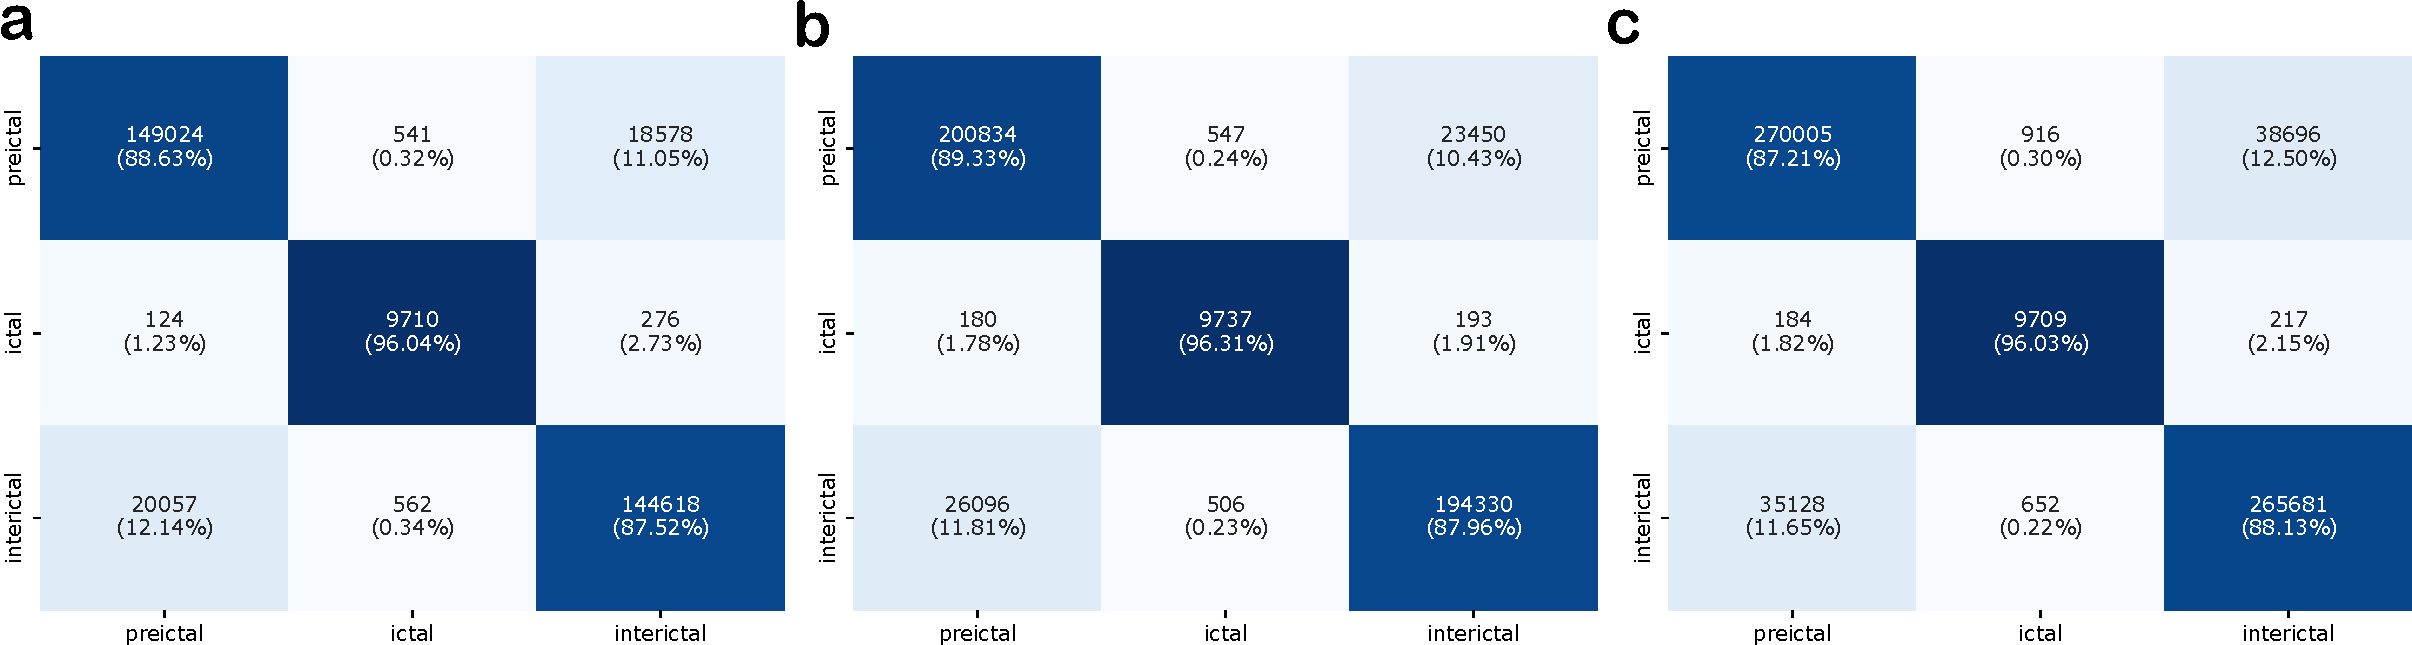
\includegraphics[width=\linewidth]{figures/conf-lookbacks_grouped.pdf}
    \caption{\textbf{Classification results of the final model using different preictal definitions.} Confusion matrix for predictions made across all folds using a preictal window of \textbf{a} 20, \textbf{b} 30, and \textbf{c} 60 minutes. Rows refer to ground truth labels, while columns to predicted ones. Percentage values indicate the number of samples classified to a given class relative to the total number of ground truth samples in that class.}
    \label{figs2:confusion_lookbacks}
\end{figure*}

\subsection{Feature and edge explainability for multiple predictive horizons}

We computed the explainability scores both for feature and edge importance to evaluate the influence of the preictal period extension on the scores. We also computed the same inter-period differences of feature importances as for the original 10-minute preictal lookback. The results are shown in figures \ref{figs5:lookback_1200}, \ref{figs6:lookback_1800}, and \ref{figs7:lookback_3600}. It can be seen that across all horizons, connectivity changes are not visible. Similar things hold for feature importances, except the 30-minute and 60-minute lookback horizons. In these cases, we observe changes in the preictal predictions, especially for the 60-minute lookback. Overall, the score of all features decreases, and the most relevant features change. Katz FD gains importance relative to the other features. We speculate that these changes can be related to the observed drops in predictive performance for the more distant samples, indicating that the network starts using different indicators of these activities. We leave the in-depth analysis for further research.

\begin{figure}[h]
    \centering
    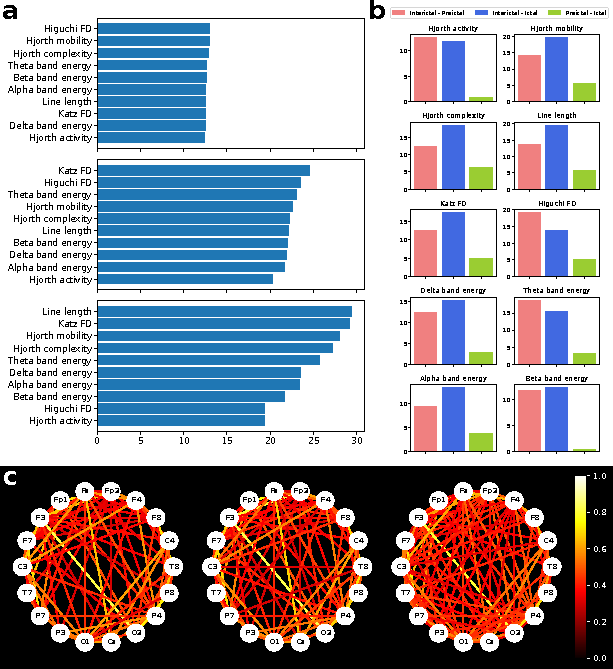
\includegraphics[width=\linewidth]{figures/lookback_1200.pdf}
    \caption{\textbf{Feature importance for experiments with the interictal horizon of 20 minutes.} Top right: average node feature importance scores obtained from predictions on every sample across all folds. \textbf{a} interictal class, middle: preictal class, bottom: ictal class. \textbf{b} Differences in importance scores between predictions for chosen classes. \textbf{c} Edge importance scores based on attention coefficients obtained from predictions on every sample across all folds for different preictal horizons. Edges with attention scores below 0.2 are not shown for clarity. Self-loops are not visualized. Left: interictal class; center: preictal class; right: ictal class.}
    \label{figs5:lookback_1200}
\end{figure}

\begin{figure}[h]
    \centering
    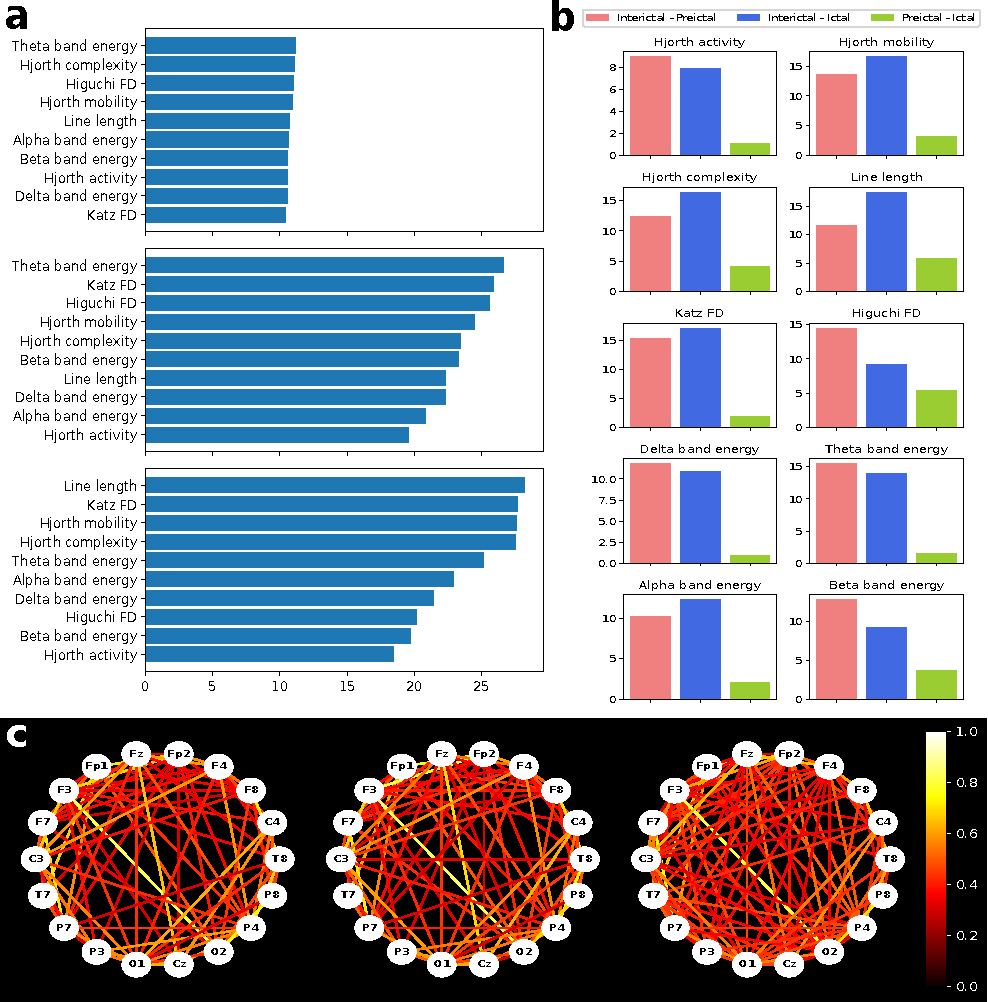
\includegraphics[width=\linewidth]{figures/lookback_1800.pdf}
    \caption{\textbf{Feature importance for experiments with the interictal horizon of 30 minutes.} Top right: average node feature importance scores obtained from predictions on every sample across all folds. \textbf{a} interictal class, middle: preictal class, bottom: ictal class. \textbf{b} Differences in importance scores between predictions for chosen classes. \textbf{c} Edge importance scores based on attention coefficients obtained from predictions on every sample across all folds for different preictal horizons. Edges with attention scores below 0.2 are not shown for clarity. Self-loops are not visualized. Left: interictal class; center: preictal class; right: ictal class.}
    \label{figs6:lookback_1800}
\end{figure}

\begin{figure}[h]
    \centering
    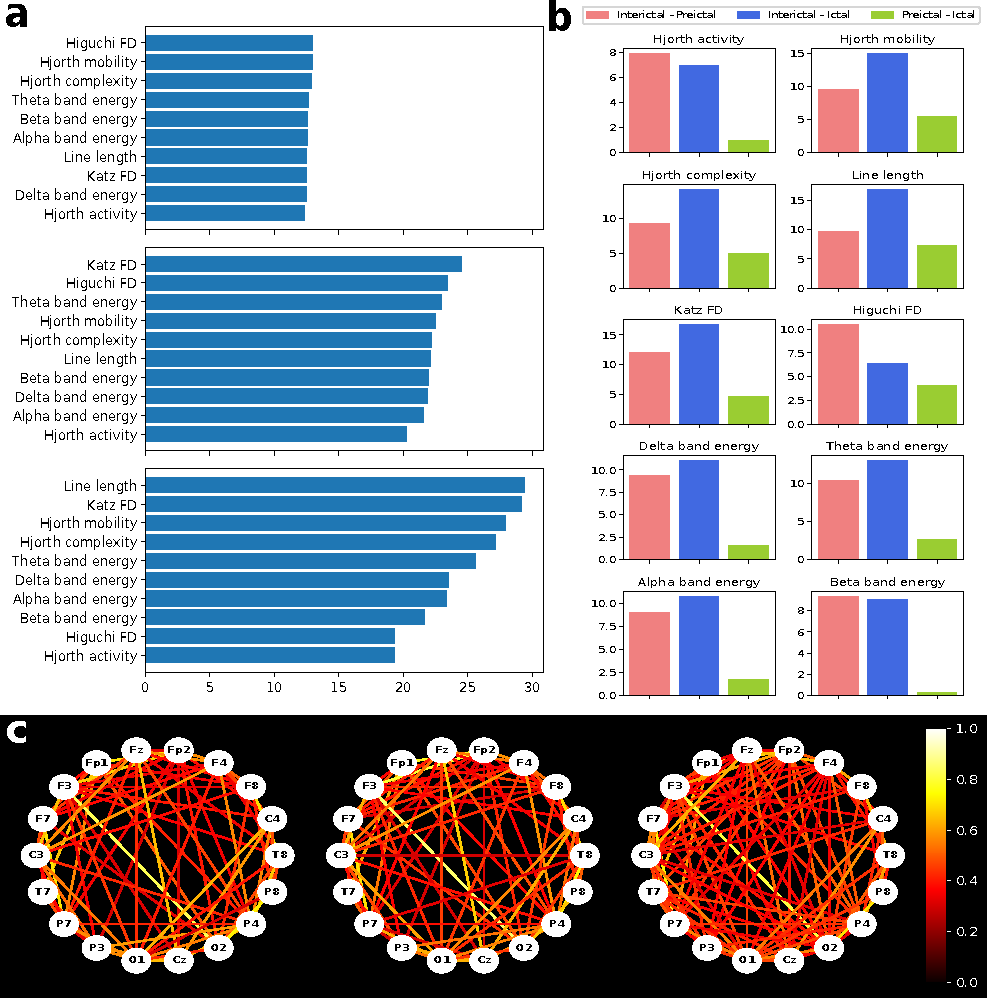
\includegraphics[width=\linewidth]{figures/lookback_3600.pdf}
    \caption{\textbf{Feature importance for experiments with the interictal horizon of 60 minutes.} Top right: average node feature importance scores obtained from predictions on every sample across all folds. \textbf{a} interictal class, middle: preictal class, bottom: ictal class. \textbf{b} Differences in importance scores between predictions for chosen classes. \textbf{c} Edge importance scores based on attention coefficients obtained from predictions on every sample across all folds for different preictal horizons. Edges with attention scores below 0.2 are not shown for clarity. Self-loops are not visualized. Left: interictal class; center: preictal class; right: ictal class.}
    \label{figs7:lookback_3600}
\end{figure}

\clearpage

%% Loading bibliography style file
\bibliographystyle{model1-num-names}
% \bibliographystyle{cas-model2-names}

% Loading bibliography database
\bibliography{cas-refs}

\begin{comment} % Maybe we can skip this. The papers of this journal do not have this.
%\vskip3pt
\bio{figures/szymon.jpeg}
Szymon Mazurek holds a master's degree in computer science from AGH University of Krak\'ow, where he is currently a PhD student in the same discipline. He is mainly interested in deep learning, especially graph-based, and the overall application of AI in medicine. For his PhD, he focuses on spiking neural networks and their performance enhancement with biologically plausible modulation. Currently, as a member Brain and More Lab, he works in the Sano Centre for Computational Medicine. He is also a research engineer at ACC Cyfronet AGH, where he is involved in using HPC for large-scale AI computations.
\endbio

\bio{figures/joan.png}
Joan Falc\'o Roget studied physics and biophysics at the University of Barcelona and at the Autonomous University of Madrid. He is a PhD Student at Sano Centre for Personalised Computational doing research in functional, diffusion, and effective connectivity in clinically oriented frameworks. He is also active in the field of theoretical neuroscience and has done research in normative models of animal behavior and in quantum computing solutions applied to computational neuroscience as well as medicine. This work was partly done while associated with the AGH University of Krak\'ow.
\endbio

\bio{figures/rosmary_elsvier.jpg}
Rosmary Blanco is a biotechnologist and a Neuroscience Ph.D. student at the Sano Centre for Computational Medicine. Her research focuses on investigating brain dynamics using diverse models, methods, and techniques, including EEG and fNIRS, to understand the large-scale network principles governing neuronal communication, cognition, and human behavior. She also integrates emerging technologies, utilizing wearable devices as cost-effective solutions for real-world neurophysiological investigations to support decision-making in the diagnostic process.
\endbio

\bio{figures/alex.jpeg}
Dr. Alessandro Crimi completed his studies in engineering at the University of Palermo,  obtained a PhD in machine learning applied for medical imaging from the University of Copenhagen,  and an MBA in healthcare management from the University of Basel. Alessandro worked as a post-doctoral researcher at the French Institute for Research in Computer Science (INRIA), the Technical School of Switzerland (ETH-Zurich), the Italian Institute for Technology (IIT), and the University Hospital of Zurich. In those institutes, he made significant contributions to the field of computational neuroscience. He taught for 8 years at the African Institute for Mathematical Science (AIMS) in Ghana and South Africa the course of machine learning in medicine, where he also supervised numerous MSc theses. Currently, he is a research group leader at Sano Centre for Computational Medicine and an associate professor at the AGH University of Krak\'ow in Poland. Dr. Crimi is also currently involved in initiatives to promote entrepreneurship with women and individuals with immigrant backgrounds, as well as technology transfer projects for young scientists.
\endbio
\end{comment}

\end{document}

